%%
%% Copyright 2007-2019 Elsevier Ltd
%%
%% This file is part of the 'Elsarticle Bundle'.
%% ---------------------------------------------
%%
%% It may be distributed under the conditions of the LaTeX Project Public
%% License, either version 1.2 of this license or (at your option) any
%% later version.  The latest version of this license is in
%%    http://www.latex-project.org/lppl.txt
%% and version 1.2 or later is part of all distributions of LaTeX
%% version 1999/12/01 or later.
%%
%% The list of all files belonging to the 'Elsarticle Bundle' is
%% given in the file `manifest.txt'.
%%

%% Template article for Elsevier's document class `elsarticle'
%% with numbered style bibliographic references
%% SP 2008/03/01
%%
%%
%%
%% $Id: elsarticle-template-num.tex 168 2019-02-25 07:15:41Z apu.v $
%%
%%
\documentclass[preprint,review,12pt]{elsarticle}
\biboptions{sort&compress}

%% Use the option review to obtain double line spacing
% \documentclass[authoryear,preprint,review,12pt]{elsarticle}

%% Use the options 1p,twocolumn; 3p; 3p,twocolumn; 5p; or 5p,twocolumn
%% for a journal layout:
%% \documentclass[final,1p,times]{elsarticle}
% \documentclass[final,1p,times,twocolumn]{elsarticle}
%% \documentclass[final,3p,times]{elsarticle}
% \documentclass[final,3p,times,twocolumn]{elsarticle}
%% \documentclass[final,5p,times]{elsarticle}
%% \documentclass[final,5p,times,twocolumn]{elsarticle}

%% For including figures, graphicx.sty has been loaded in
%% elsarticle.cls. If you prefer to use the old commands
%% please give \usepackage{epsfig}

%% The amssymb package provides various useful mathematical symbols
\usepackage{amssymb}
%% The amsthm package provides extended theorem environments
% \usepackage{amsthm}

%% The lineno packages adds line numbers. Start line numbering with
%% \begin{linenumbers}, end it with \end{linenumbers}. Or switch it on
%% for the whole article with \linenumbers.
%% \usepackage{lineno}

%%!!!!user's commands
\usepackage{amsmath}
\newcommand{\angstrom}{\text{\normalfont\AA}}

\newcommand{\hmn}[1]{% Hermann-Maguin notation
  \ensuremath{\begingroup\setupHMN #1\endgroup}%
}

\newcommand{\setupHMN}{%
  \doHMN{-}{\HMNoverline}%
  \doHMN{*}{\HMNminverse}%
  \doHMN{i}{\infty}
}

\newcommand{\doHMN}[2]{%
  \begingroup\lccode`~=`#1
  \lowercase{\endgroup\let~}#2%
  \mathcode`#1="8000
}

\newcommand{\HMNminverse}[1]{\frac{#1}{m}}
\newcommand{\HMNoverline}[1]{\mkern1mu\overline{\mkern-1mu#1\mkern-1mu}\mkern1mu}

\usepackage{miller}
\usepackage{multirow}
\usepackage{xcolor}
\usepackage{subfigure}
\usepackage[breaklinks]{hyperref}
\usepackage{graphicx}

\journal{Journal of Solid State Chemistry}

\begin{document}

\begin{frontmatter}

%% Title, authors and addresses

%% use the tnoteref command within \title for footnotes;
%% use the tnotetext command for theassociated footnote;
%% use the fnref command within \author or \address for footnotes;
%% use the fntext command for theassociated footnote;
%% use the corref command within \author for corresponding author footnotes;
%% use the cortext command for theassociated footnote;
%% use the ead command for the email address,
%% and the form \ead[url] for the home page:
%% \title{Title\tnoteref{label1}}
%% \tnotetext[label1]{}
%% \author{Name\corref{cor1}\fnref{label2}}
%% \ead{email address}
%% \ead[url]{home page}
%% \fntext[label2]{}
%% \cortext[cor1]{}
%% \address{Address\fnref{label3}}
%% \fntext[label3]{}

\title{Laves polyhedra in synthetic tennantite, Cu\textsubscript{12}As\textsubscript{4}S\textsubscript{13}, and its lattice dynamics}

\author[TISNCM]{Alexey~A.~Yaroslavzev}
\ead{yaroslavzevalex@gmail.com}
\author[MSU,ICRAS]{Alexey~N.~Kuznetsov}
\author[SIC]{Alexander~P.~Dudka}
\author[MSU]{Andrei~V.~Mironov}
\author[TISNCM]{Sergey~G.~Buga}
\author[TISNCM]{Vladimir~V.~Denisov}

\address[TISNCM]{Technological Institute for Superhard and Novel Carbon Materials, 108840, Troitsk, Moscow, Russia}
\address[MSU]{Department of Chemistry, Lomonosov Moscow State University, 119991, Moscow, Russia}
\address[ICRAS]{Kurnakov Institute of General and Inorganic Chemistry RAS, 119991, Moscow, Russia}
\address[SIC]{Shubnikov Institute of Crystallography of Federal Scientific Research Centre “Crystallography and Photonics” of Russian Academy of Sciences, Leninskiy Prospekt 59, 119333, Moscow, Russia}


\begin{abstract}
Synthetic tennantite, Cu\textsubscript{12}As\textsubscript{4}S\textsubscript{13}, is the analogue of an abundant mineral that belongs to the tennantite-tetrahedrite group with a low lattice thermal conductivity.
Combined data from high-quality X-ray diffraction, electron microscopy (STEM--HAADF), Raman spectroscopy, as well as DFT calculations are used to analyze the peculiarities of its structure stability and dynamics.
Atomic displacement parameters (ADP) and low-energy optical phonon modes are discussed within the context of the structure variations and pecularities of the charge distribution.
The latter indicates that the tennantite structure tends to conform to the covalent polar bonds and its charge distribution is significantly affected by the atomic shifts in Laves polyhedra.
According to the DFT calculations, there is a population of stable model structures with varying shifts of copper atoms in Laves polyhedra, with total energies being very close (within 0.24~eV), which can explain the observed behavior of the ADP.
A specially designed  technique is used for the experimental analysis of the ADP that revealed Einstein characteristic temperatures in the tennantite structure to be in the range of 50--190~K, which is attributed to  low-energy optical phonon modes.


\section*{Highlights}
\begin{itemize}
  \item Synthetic tennantite Cu\textsubscript{12}As\textsubscript{4}S\textsubscript{13} structure consists of disordered Laves polyhedra
  \item DFT calculations reveal a mixed valence of Cu atoms, and Laves polyhedra distortions
  \item Jahn-Teller distortions give rise to a set of unit cells with close ground state energies
  \item Rattling vibration modes refer to Einstein temperatures of 74, 104, 115, 185K
\end{itemize}

\end{abstract}

\begin{keyword}
tennantite Cu\textsubscript{12}As\textsubscript{4}S\textsubscript{13}\sep
thermoelectic materials\sep
DFT calculations\sep
structural anisotropy\sep
Raman spectroscopy\sep
X-ray diffraction\sep
computer simulations\sep

%% PACS codes here, in the form: \PACS code \sep code

%% MSC codes here, in the form: \MSC code \sep code
%% or \MSC[2008] code \sep code (2000 is the default)

\end{keyword}

\end{frontmatter}

%% \linenumbers

%% main text
% \section{}
% \label{}
\section{Introduction}\label{sec:level1}

The tennantite-tetrahedrite group represents a large class of inorganic compounds, including complex copper sulfosalts with the general formula Cu\textsubscript{10+x}M\textsubscript{2-x}X\textsubscript{4}S\textsubscript{13}, where M is a transition metal (Zn, Fe, Hg, etc.), and X is a pnictogen (As, Sb, or Bi) \cite{Makovicky_2006}, with the pure tennantite itself represented by the formula Cu\textsubscript{12}As\textsubscript{4}S\textsubscript{13}.
Despite being known for over two centuries, these minerals still represent objects of intense studies, both due to  structural peculiarities and potential applications. Arsenic- and antimony-containing compounds of this class are considered as advanced thermoelectric materials with a low lattice thermal conductivity\cite{Sootsman2009,Chetty2015}.
For instance, tetrahedrite doped with Mn, Fe, Co, Ni, Zn, Te, Se showed ZT values in the range from 0.2 to 1.13\cite{Heo2014,Suekuni2013,Lu2012,Barbier2016,Rout2020,Zhu2019}.

The tennantite structure is treated as a sphalerite-type, thus conforms to the \hmn{I -4 3 m} space group\cite{yaroslavzev2019,Makovicky_2006}.
The structure can be described by five nonequivalent crystallographic sites: two for Cu, one for As, and two for S.
Cu1 is tetrahedrally coordinated (CuS\textsubscript{4}) by four S1, and As forms a trigonal pyramid (AsS\textsubscript{3}) with three S1.
Additionally, the S2 is a center of an octahedral unit that is called a Laves polyhedra (SCu\textsubscript{6}) with six copper atoms in sites Cu2 and Cu21.
Cu2 is trigonally coordinated (CuS\textsubscript{3}) by two S1 and one S2, while Cu21 is coordinated by two S1, one S2 and one As atoms.
Cu21 and Cu2 atoms show very large atomic displacements perpendicular to the plane of the triangle (Fig.~\ref{fig:generel_view}, right).

In a case of tennantite- and tetrahedrite-based materials, it is generally considered that a low lattice thermal conductivity is caused by hybridized Cu {\it 3d}  and chalcogen {\it p} orbitals\cite{Lai2015}.
Such a hybridization leads to a bonding asymmetry, and out-of-plane low frequency rattling modes, which are quasi-localized and anharmonic\cite{May2016,Bouyrie2015}.

\begin{figure}[ht]
\centering
\subfigure{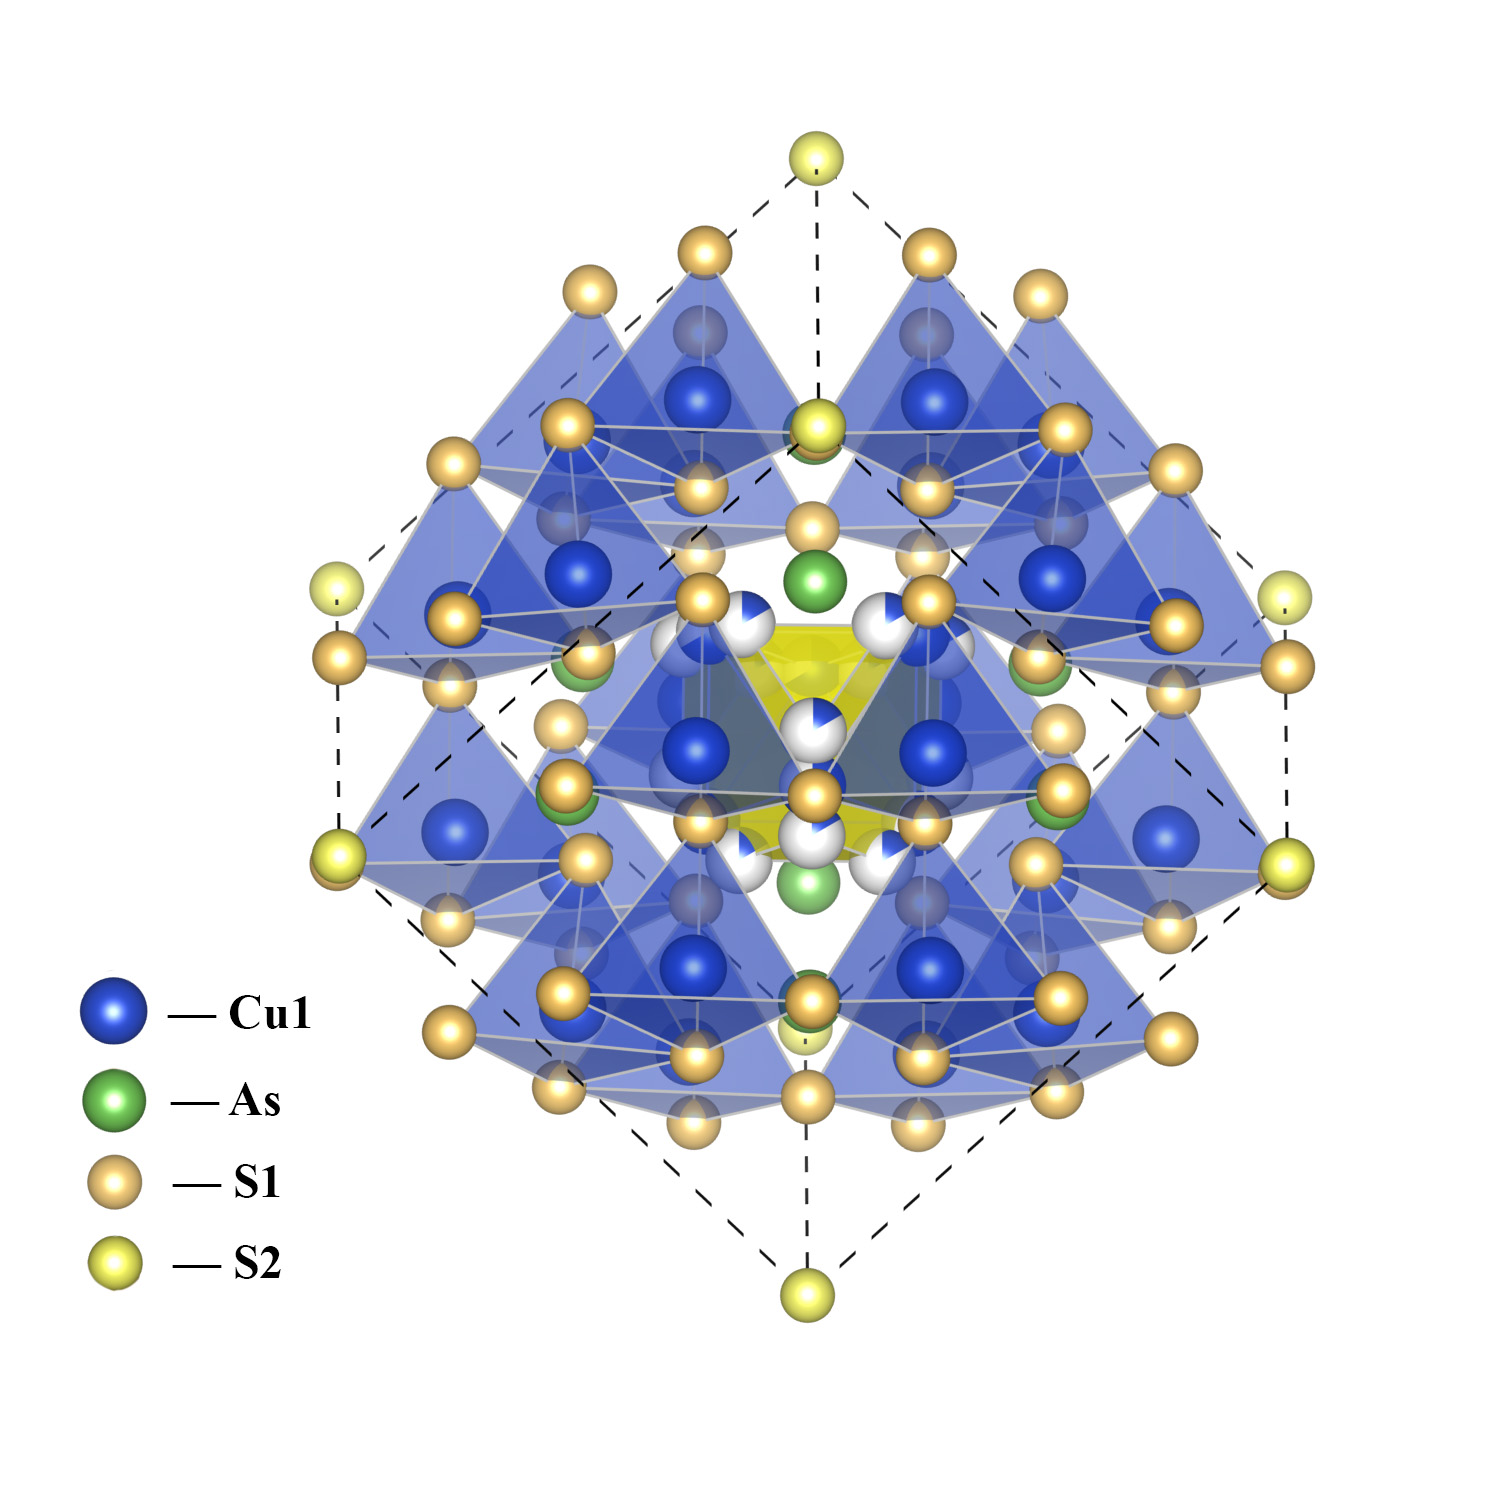
\includegraphics[width=0.4\columnwidth]{general_view}}
 \quad
\subfigure{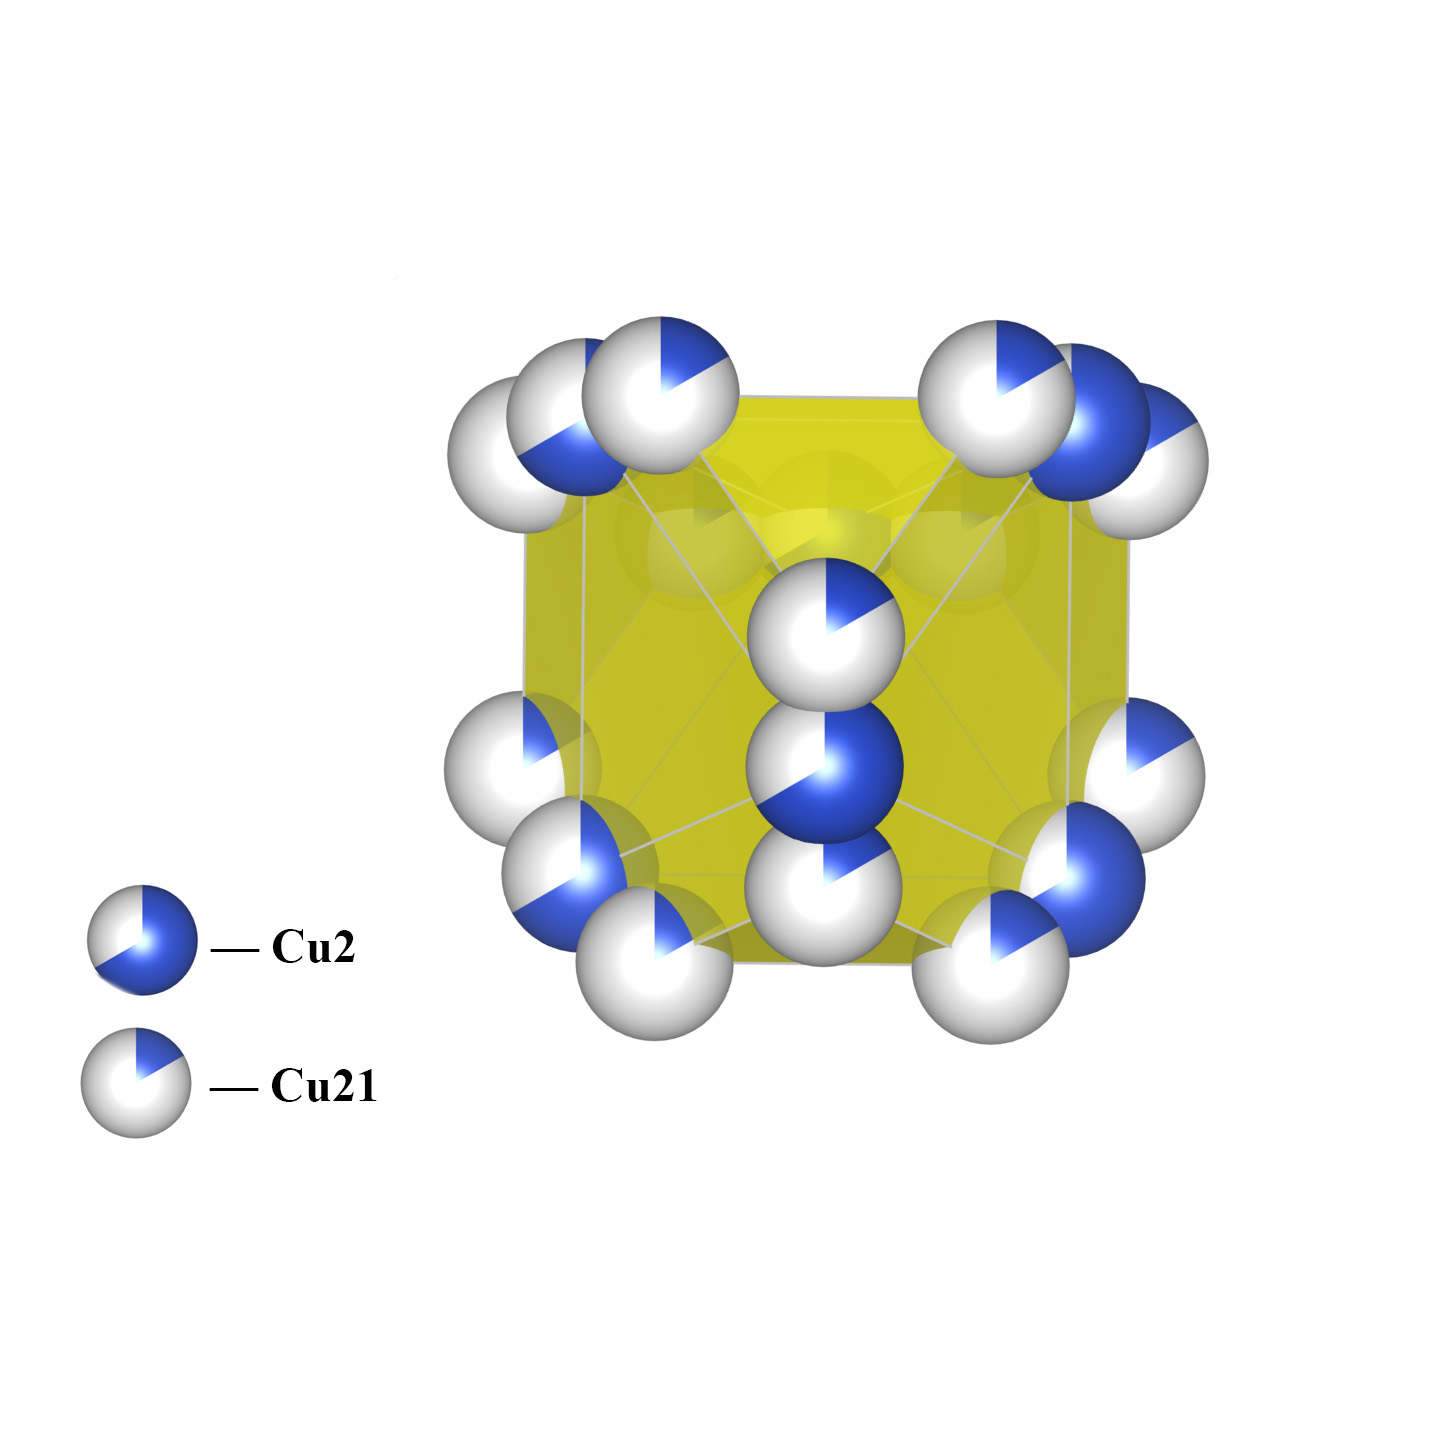
\includegraphics[width=0.35\columnwidth]{general_view_laves}}
\caption{\label{fig:generel_view} Left --- the Cu\textsubscript{12}As\textsubscript{4}S\textsubscript{13} tennantite structure with coordination polyhedra around the Cu1 (blue), and the Laves polyhedra (yellow); right --- the Laves polyhedra containing Cu2 and Cu21 atoms with their partial occupancies shown as sections of spheres.}
\end{figure}

Some authors note\cite{DiBenedetto2005,Tanaka2015}, that asymmetric bonds give rise to magnetic properties and, in some cases, to antiferromagnetic (AFM) ordering\cite{yaroslavzev2019,Blandy_2018}.
In both kinds of materials, deviations from the Curie-Weiss law in the temperature dependencies of the magnetization were revealed: at 124~K\cite{Tanaka2015} in tennantite, and at 84~K\cite{Nasonova2016_2} in tetrahedrite.

According to the structural study, these deviations take place due to the distortion of Cu\textsubscript{6}S octahedra (Laves polyhedra)\cite{Tanaka2015}.
The distortion at 84 K in tetrahedrite is reported to lead to either the symmetry lowering from \hmn{I -4 3 m} to \hmn{I -4 2 m}  space group accompanied by the displacement of S atoms\cite{Hathwar2019}, or to a shift of Cu2 atoms towards S\textsubscript{3} triangle plane with S\textsubscript{2} displacement\cite{Nasonova2016_2} in the same symmetry, and space group.

Recently, we have performed a multi-temperature (90--298~K) structural study of a synthetic tennantite\cite{yaroslavzev2019} and found that below ca. 120 K the copper atom distribution in tennantite changes from a more statistically delocalized Cu2 to a well-defined split into Cu2 and Cu21 positions without a first-order phase transition.
This effect is accompanied by As1 and S2 atoms displacement, which was also observed in Ref.~\cite{Hathwar2019}.
We also investigated the low- and room-temperature electronic structures of a synthetic tennantite based on the DFT calculations, which confirmed the second-order transition from the low-temperature AFM to the room-temperature PM state\cite{yaroslavzev2019}.

However, the relationships between the peculiarities of the tennantite crystal and its electronic structures and thermoelectric properties, including the behavior of Laves polyhedra in the structure, were put aside in the previous paper\cite{yaroslavzev2019}.
In this paper, we focus on these problems, and  investigate the tennantite cell energy distribution, and the charge density differences for different Cu positions in the Laves polyhedra.
Also, we investigate low-energy phonon modes, and peculiarities of the ADP in the temperature range of 85--293~K, the same as in Ref.~\cite{Dudka2019}, in the context of the cell energy distribution.
To clarify the distortions in Laves polyhedra, a study of the spherical single-crystal sample was performed and the high-angle annular dark-field (HAADF) images were obtained.


\section{Materials and methods}\label{sec:level1}
\subsection{Synthesis}\label{sec:level2}

High quality single crystals of Cu\textsubscript{12}As\textsubscript{4}S\textsubscript{13} for the XRD analysis were grown using a two-step procedure. At first, bulk Cu\textsubscript{12}As\textsubscript{4}S\textsubscript{13} has been prepared by a high-temperature technique from copper (99.5~\%), arsenic (99.5~\%), and sulphur (99.5~\%).
Then, the ingots were subjected to directional recrystallization by the Bridgman-Stockbarger technique in a two-zone furnace.
The temperature in the recrystallization zone was chosen 40 K~above the tennantite melting point. A speed of the ingot motion was set at 0.5~mm/hour, with the temperature gradient in the recrystallization zone ca.~8--10~K/mm.

\subsection{Single-crystal X-ray diffraction}\label{sec:level2}
A spherically shaped single-crystal sample of Cu\textsubscript{12}As\textsubscript{4}S\textsubscript{13}  was prepared for the anisotropic extinction study\cite{Becker1975}.
Enraf-Nonius CAD-4 diffractometer with AgK\textsubscript{$\alpha$} equipped with graphite monochromator was used for the data collection.
The spherical single-crystal structural study results are presented in Supplementary Material, and they are compared with the structural data from the regularly shaped crystal sample\cite{yaroslavzev2019}.

\subsection{Analysis of temperature dynamics of atomic displacements}\label{sec:level2}
The temperature dynamics of an atomic displacement from the previous study\cite{yaroslavzev2019} were used to estimate Einstein characteristic temperatures by the mixed Einstein-Debye model using DebyeFit program\cite{Dudka2019}.
The data are based on the study of  Cu\textsubscript{12}As\textsubscript{4}S\textsubscript{13} single-crystal sample at 85, 115, 180, 250, and 293~K.
The sample has a rectangular shape with the dimensions of 0.456~$\times$~0.31~$\times$~0.247~mm\textsuperscript{3}.
Xcalibur diffractometer equipped with a CCD EOS S2 detector (Rigaku Oxford Diffraction, MoK\textsubscript{$\alpha$}) and Cobra Plus (Oxford Cryosystems) apparatus with nitrogen gas flow combination were used for the data collection.
The original experimental methods and data processing are presented in Supplementary Material in details.

\subsection{Theoretical calculations}\label{sec:level2}
Calculations on the stability of possible tennantite polytypes were performed based on Density Function Theory (DFT)\cite{Kohn1965} within the generalized gradient approximation (GGA) using Perdew-Burke-Ernzerhof exchange-correlation functional\cite{Perdew1996}.
We used the projector augmented wave method\cite{Blchl1994} with the periodic boundary conditions as implemented in Vienna Ab-initio Simulation Package (VASP)\cite{Kresse1996,Kresse1996-2,Kresse1993,Kresse1994}.
The plane-wave energy cut-off was set to 450~eV. To calculate the equilibrium atomic structure, the Brillouin zone was sampled according to the Monkhorst–Pack scheme\cite{Monkhorst1976} with a 6$\times$6$\times$6 grid in the {\it k}-space. The convergence criterion for the structural relaxation was set at 0.1~meV.
Both the unit cell symmetry and parameters were allowed to relax.
To facilitate unconstrained structural optimization, all the starting structures were converted to \hmn{P1} space group.


\subsection{Electron microscopy}\label{sec:level2}
High-resolution electron microscopy images were taken using FEI~Titan~80--300 transmission electron microscope in the HAADF--STEM mode (high-angle annular dark-field scanning transmission) with an acceleration voltage of 300~kV. The sample for microscopy was prepared using FEI~Helios~600 focused ion beam setup. HAADF image was fitted by Atomap\cite{Nord2017} package written in Python.

\subsection{Raman Spectroscopy}\label{sec:level2}
Raman spectroscopy study was performed with a spectrometer TRIAX-552, equipped with Peltier TE-cooled detector CCD~SPEC~10~(Princeton Instruments).
A grating of 600~lines~mm\textsuperscript{-1}, and a 50\textsuperscript{$\times$} lens Mitutoyo~M~Plan~Apo~SL50 (a numerical aperture of 0.42) were used. Raman spectra was excited with 514.5~nm argon-ion laser Spectra-Physics Stabilite 2017 with 1~mW output power on a sample. An open argon gas flow was used to reduce air’s modes.
Calibration was performed using 520.5~cm\textsuperscript{-1} Raman peak of a polished silicon wafer. 
We used 3~ONDAX~114-ER297-001 fiber Bragg gratings to observe lines near the laser one. Fittings of the Raman spectra were performed by the LMFIT\cite{LMFIT} package written in Python. The fitting model was based on 6 pseudo-Voigt functions and a polynomial function for the background.

\section{Results and discussion}\label{sec:level1}

\subsection{Remarks on the structure of synthetic tennantite}\label{sec:level2}
The study of the high quality single crystal allowed us to re-investigate the crystal structure of Cu\textsubscript{12}As\textsubscript{4}S\textsubscript{13}  with a high precision.
The structure was refined in a way similar to previously described in Ref.~\cite{yaroslavzev2019}.
The sum of occupancies for Cu2, Cu21 and its symmetry related site were constrained to 1.
Due to rather large distance between these atoms their ADP were refined independently.
The maximum entropy method (MEM) refinement gave the result identical to \cite{yaroslavzev2019}.
Our data confirms that the compound contains 12 copper atoms per formula unit, and shows no evidence of copper deficiency.
Neither XRD, nor TEM data have shown detectable packing defects.

\begin{table}
\caption{\label{tab:anis_ext}%
Anisotropic extinction parameters in Cu\textsubscript{12}As\textsubscript{4}S\textsubscript{13}.
}
\centering
\resizebox{\columnwidth}{!}{
\begin{tabular}{cccccc}

\textrm{ g\textsubscript{11}$\times$10\textsuperscript{4}}&
\textrm{ g\textsubscript{22}$\times$10\textsuperscript{4}}&
\textrm{ g\textsubscript{33}$\times$10\textsuperscript{4}}&
\textrm{ g\textsubscript{12}$\times$10\textsuperscript{4}}&
\textrm{ g\textsubscript{13}$\times$10\textsuperscript{4}}&
\textrm{ g\textsubscript{23}$\times$10\textsuperscript{4}}  \\
1.4(4)	& 4.2(8)	& 2.7(4)	& 1.0(3) &	0.2(3)	& -1.1(5) \\
\end{tabular}}
\end{table}

Due to the crystal growth method used, the sample shows a degree of anisotropic extinction. Extinction parameters are presented in the Table~\ref{tab:anis_ext}.
The disorder of Cu21 is observed in the analyzed HAADF image of the sample in [110] zone (Fig.~\ref{fig:micro}).
The electron diffraction, and overlay of HAADF image with the tennantite crystal [110] zone generated by VESTA\cite{Momma2011}, are given in Supplementary Material.
Processed HAADF image (Fig.~\ref{fig:micro}, right) shows  an ellipticity for the Cu/As atomic columns, which is a measure of the atomic column elongation\cite{Nord2017}.
The atomic column elongation is evidenced by the blurring of the intensity distribution, and a large atomic displacement.
Similar effects were observed in tetrahedrite\cite{Mishra2017}, and several tetrahedral framework structures\cite{Suekuni2019}.
Also, the observed anisotropic displacement may possibly be caused by the crystal growth conditions or/and a crystal cell distortion.
However, in such case the structure must show prominent diagonal distortion and/or feature an increase or decrease of the copper content per cell (with respect to 12 copper atoms), which is not the case.

\begin{figure}[ht]
\centering
\subfigure{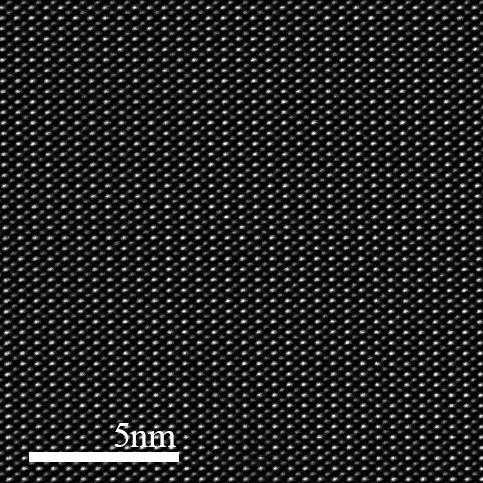
\includegraphics[width=0.35\columnwidth]{mic_Figure_10}}
 \quad
\subfigure{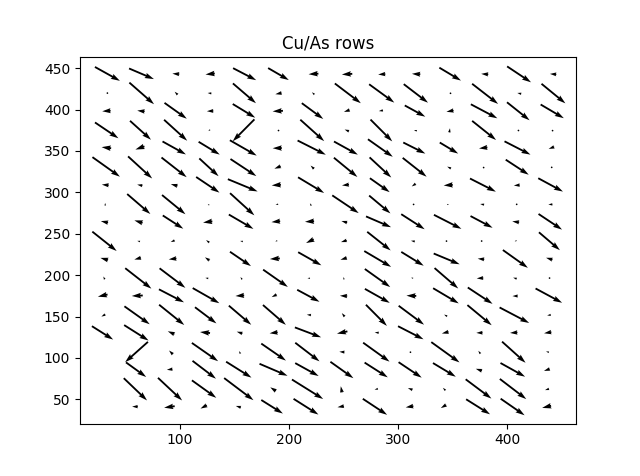
\includegraphics[width=0.49\columnwidth]{CuAs_raws_normal}}
\caption{\label{fig:micro} Left --- the HAADF image of tennantite crystal viewed from the [110] zone; right --- the processed HAADF image with the ellipticity for the Cu/As atomic columns. The analysis implied quantifying the positions and shapes of atomic columns based on Atomap\cite{Nord2017}. }
\end{figure}


\subsection{Atomic displacement parameter temperature dynamics analysis based on diffraction data}\label{sec:level2}

The ADP were analyzed by DebyeFit program using the crystallographic data.
The DebyeFit estimates the Debye or/and Einstein characteristic temperature in crystals from the equivalent ADP obtained at different temperatures.

At fitting, ADPs are considered as a combination of quantum zero vibrations, thermal vibrations, and static shifts\cite{Trueblood1996,Bentien2005,Nakatsuka2011}.
The thermal expansion of the crystal, and the corresponding change of the atomic vibration frequencies depend on the temperature, and may be described using a quasi-harmonic approximation\cite{willis1975thermal,Bentien2005}.
As a result, ADP is described by u\textsubscript{calc}~$=$~xu\textsubscript{E}+(1-x)u\textsubscript{D}+u\textsubscript{static}, where xu\textsubscript{E} and (1-x)u\textsubscript{D} are Einstein and Debye parts, u\textsubscript{static} is a static shift of an atom from its site in the structure model\cite{Dudka2019}.
The result of tennantite ADP fitting is presented in the Fig.~\ref{fig:enst_temp}, and Table~\ref{tab:enst_temp}.
The average oscillation frequency of the selected atom, and its characteristic Einstein temperature, T\textsubscript{E}, can be obtained  assuming x~$=$~1.
The maximal oscillation frequency of the selected atom and its characteristic Debye temperature, T\textsubscript{D}, corresponds to the case x~$=$~0.
Distributions of zero-point oscillations, u\textsubscript{0E} or u\textsubscript{0D}, were obtained applying T~$=$~0 in the Einstein or Debye formulas.
Thus, the contribution of Einstein or Debye parts to atomic displacements consists of zero quantum vibrations, u\textsubscript{0E} or u\textsubscript{0D}, and a temperature-dependent part, u\textsubscript{E}(T) or u\textsubscript{D}(T), which can be associated with the thermal motion of atoms.
That is, u\textsubscript{E} = u\textsubscript{0E} + u\textsubscript{E}(T), and u\textsubscript{D} = u\textsubscript{0D} + u\textsubscript{D}(T). The shift of an atom from its equilibrium position due to any reason other than thermal vibrations is the sum of zero vibrations and static shift: u\textsubscript{shift} = u\textsubscript{0E} + u\textsubscript{static} or u\textsubscript{shift} = u\textsubscript{0D} + u\textsubscript{static}\cite{Dudka2019}.

A good agreement between model ADP, u\textsubscript{calc}, and equivalent experimental ADP, u\textsubscript{eq}, can be obtained only if (1) the temperature of the crystal is correctly determined during the measurements; (2) the static shift of the atoms is taken into account, i.e. when using the extended model with  inclusion u\textsubscript{static} term. The fitting results are presented in Figure~\ref{fig:enst_temp}.

\begin{figure}[ht]
\centering
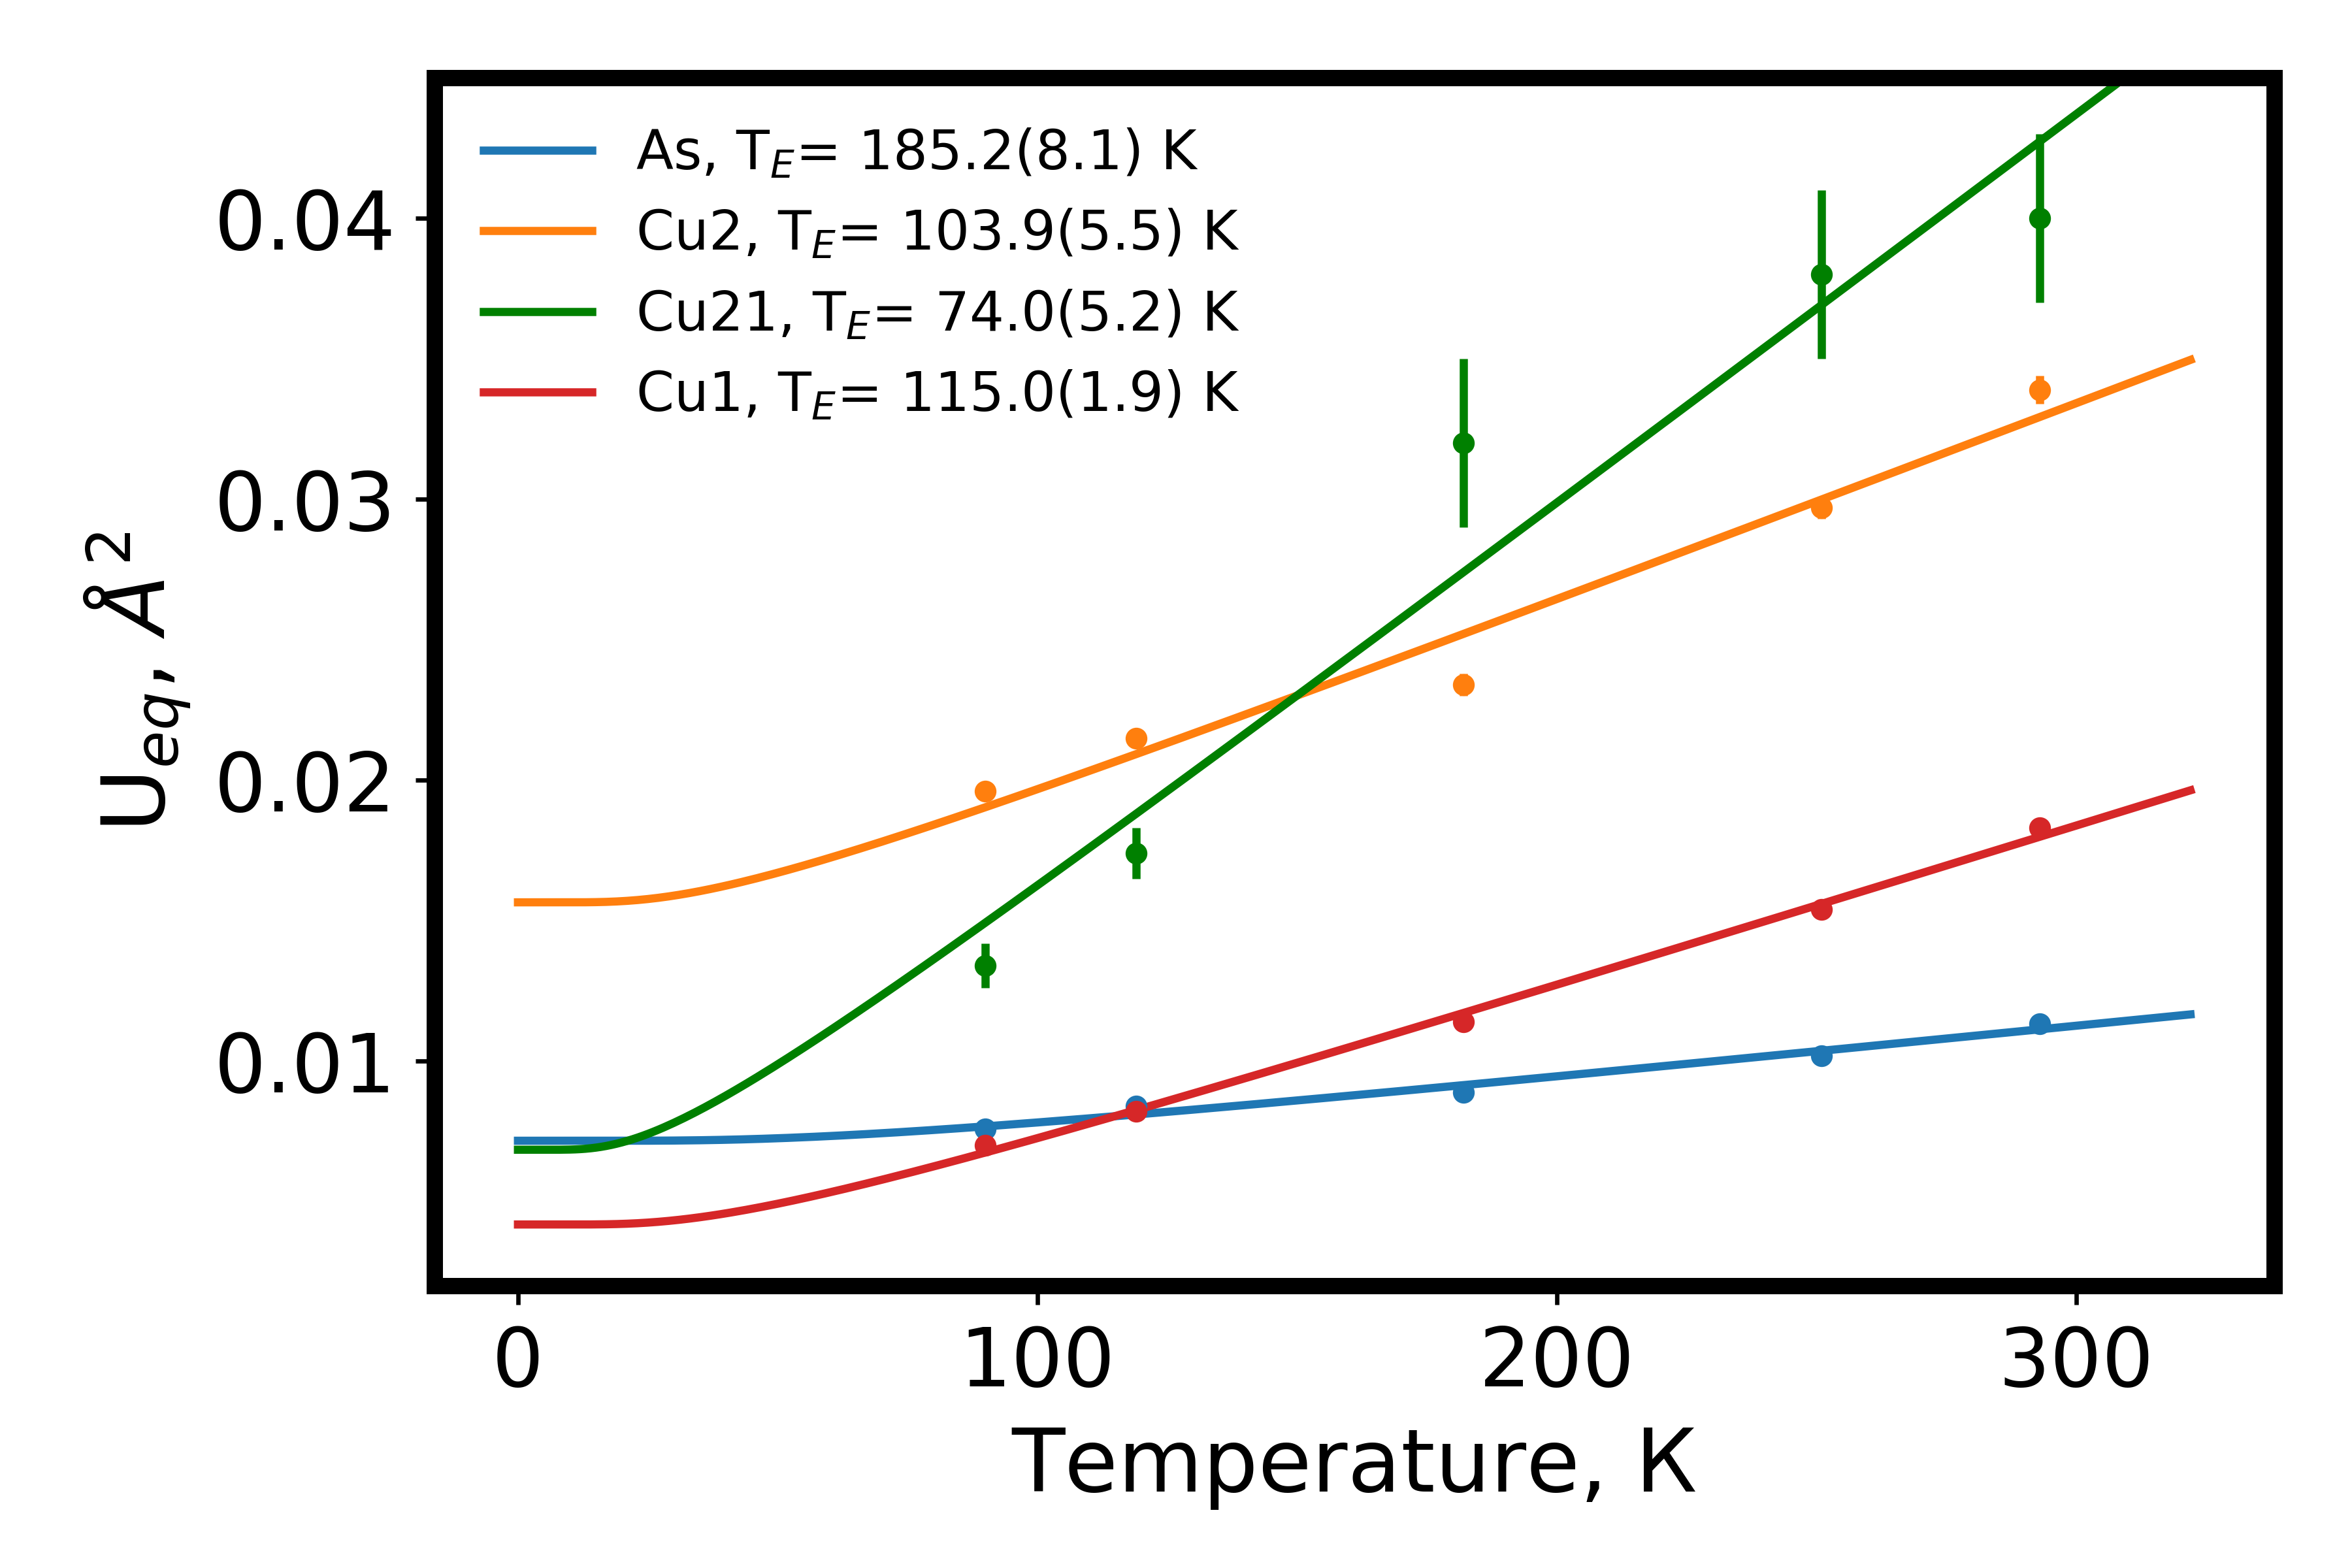
\includegraphics[width=0.48\textwidth]{ADP_aproximation_eng}% Here is how to import EPS art
\caption{\label{fig:enst_temp} Equivalent parameters u\textsubscript{eq} of the mean-square displacements of atoms in tennantite. Points are the experimental data. Solid curves show the fit of the temperature dependences according to the expanded Einstein model.}
\end{figure}

Large static values for Cu2 atom (Table~\ref{tab:enst_temp}) confirmed instability of this site\cite{Hathwar2019,yaroslavzev2019}.
This disorder is reliably described by the anharmonic model of atomic displacements using the Gram-Charlier expansion to the 4th order.

\begin{table}
\caption{\label{tab:enst_temp}
Einstein temperatures, dispersions of zero-point oscillations u\textsubscript{E$_{0}$} u\textsubscript{static}, and u\textsubscript{shift} for atoms in tennantite. $R=\sum |u\textsubscript{eq} - u\textsubscript{calc} |/\sum u\textsubscript{eq}$ is the residual factor of the LS procedure.
}
\centering
\resizebox{\columnwidth}{!}{
\begin{tabular}{cccccc}

&
\textrm{ T(Einstein)~K, cm\textsuperscript{-1}}&
\textrm{ u\textsubscript{E}$\times$10\textsuperscript{4}, $\angstrom^{2}$  }&
\textrm{ u\textsubscript{static}$\times$10\textsuperscript{4}, $\angstrom^{2}$     }&
\textrm{ u\textsubscript{shift}$\times$10\textsuperscript{4}, $\angstrom^{2}$    }&
\textrm{ R,  \% }  \\

Cu\textsubscript{1}	  & 115.0(1.9), 79.9     & 3.3	& 0.9(0.4) & 4.2 & 	1.89 \\
Cu\textsubscript{2}	  & 103.9(5.5), 72.2  & 3.7	& 12.0(1.5) & 15.7 & 	3.28 \\
Cu\textsubscript{21}  & 74.0(5.2), 51.4	   & 5.2	& 1.7(4.0) & 6.8 & 8.06 \\
As\textsubscript{1}	  & 185.2(8.1), 128.7 & 1.7	& 5.4(0.3) & 7.2 & 	2.20 \\

\end{tabular}}
\end{table}



\subsection{Analysis of anharmonic vibrations of copper atoms through the ADP and Raman spectroscopy}\label{sec:level2}

The Raman spectrum of the crystalline tennantite consists of the following well-defined peaks: $\nu_{1}$, $\nu_{2}$, $l_{1}$, $l_{2}$ at 374.5, 340, 64, and 122 cm\textsuperscript{-1} respectively, and a broad peak $\nu_{4}$ at 320 cm\textsuperscript{-1}. Peaks between 200, and 400 cm\textsuperscript{-1} refer to (Sb, As)S\textsubscript{3} groups modes\cite{Kharbish2007}.
Position of $\nu_{3}$ was found by the spectra fitting.
The fit result is presented in Figure~\ref{fig:full_raman}, and in Table 3. Peaks below 200 cm\textsuperscript{-1} are related to the lattice dynamics\cite{Buzatu2017}.

\begin{figure}[h]
\centering
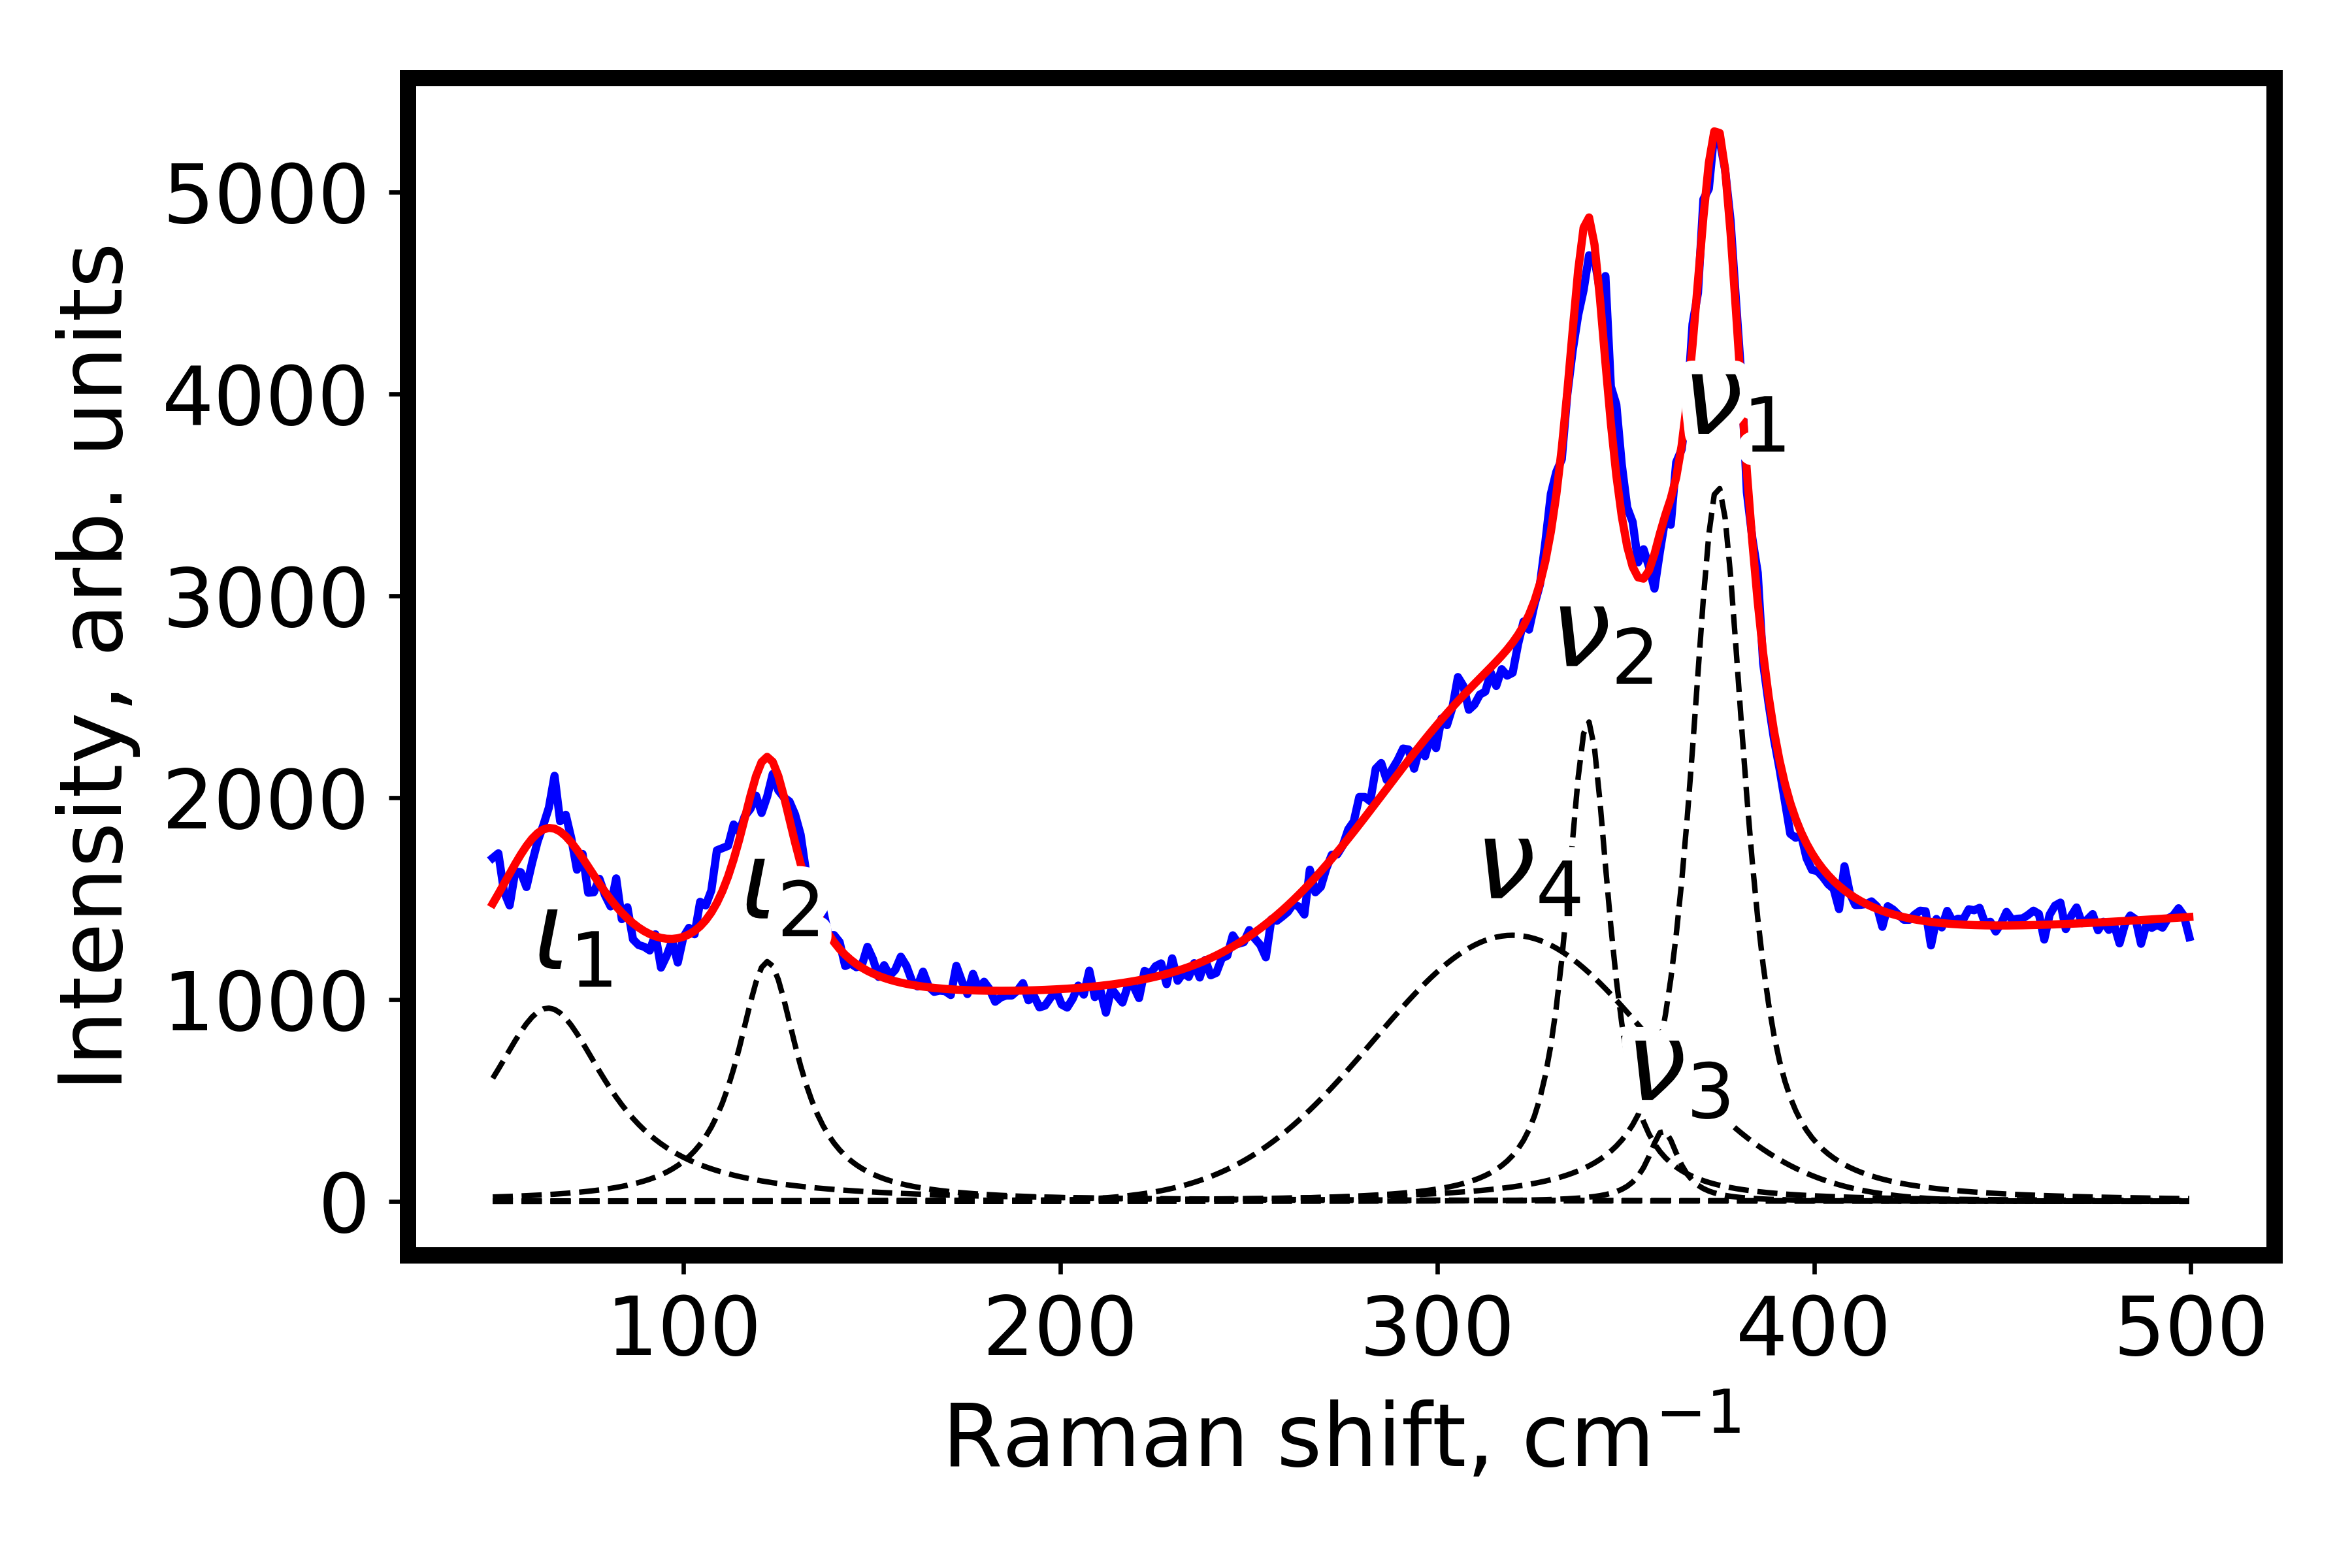
\includegraphics[width=0.48\textwidth]{raman_25_CuAsS3_eng_components}
\caption{\label{fig:full_raman} The Raman spectrum of the crystalline tennantite. Peaks between 200, and 400 cm\textsuperscript{-1} refer to (Sb, As)S\textsubscript{3} groups modes\cite{Kharbish2007}. Peaks below 200 cm\textsuperscript{-1} are related to the lattice dynamics\cite{Buzatu2017}. Blue --- experimental data, red --- the superposition of modes, dotted --- fitted peaks}.
\end{figure}

Within the approach above, the Einstein solid model is used to describe independent harmonic oscillators.
Thus, the low energy spectrum should consist of peaks with the Einstein's energies, which we found by DebyeFit (Table~\ref{tab:enst_temp}).
The results of the calculations are presented in Figure~\ref{fig:low_energ_raman}.
The Einstein's energies from structural study were used as the initial points for the fit, with the initial and fitted wavenumbers are presented and in Table~\ref{tab:ram_fit}.
The low energy $l_{1}$ and $l_{2}$ peaks are well described by Einstein's energies of Cu2, Cu21, Cu1, and As (66, 40, 79, and 122 cm\textsuperscript{-1} respectively).
Same modes were observed and analyzed in tetrahedrites\cite{May2016,Lai2015} with energies approximately 4, 9 and 18 meV (33, 72, 145 cm\textsuperscript{-1}) which is
in good agreement with our results.
Thus, we can state that the reason for the strong anharmonic behavior is a dynamic disorder of the copper atoms and arsenic atoms.
Consequently, this leads to out-of-plane low frequency rattling modes, and a low lattice thermal conductivity.


\begin{table}
\caption{\label{tab:ram_fit}
Initial and fitted Einstein's energies. Initial energies are Einstein's energies from structural study.}
\centering
\resizebox{\columnwidth}{!}{
\begin{tabular}{ccccc}
&
\textrm{ Cu2   }&
\textrm{ Cu21  }&
\textrm{ Cu1     }&
\textrm{ As    } \\

Initial Einstein's energies, cm\textsuperscript{-1}	  &  72  & 51	& 80 & 129  \\
Fitted Einstein's energies, cm\textsuperscript{-1}	  &  66  & 40	& 79 & 122  \\

\end{tabular}}
\end{table}

\begin{figure}
\centering
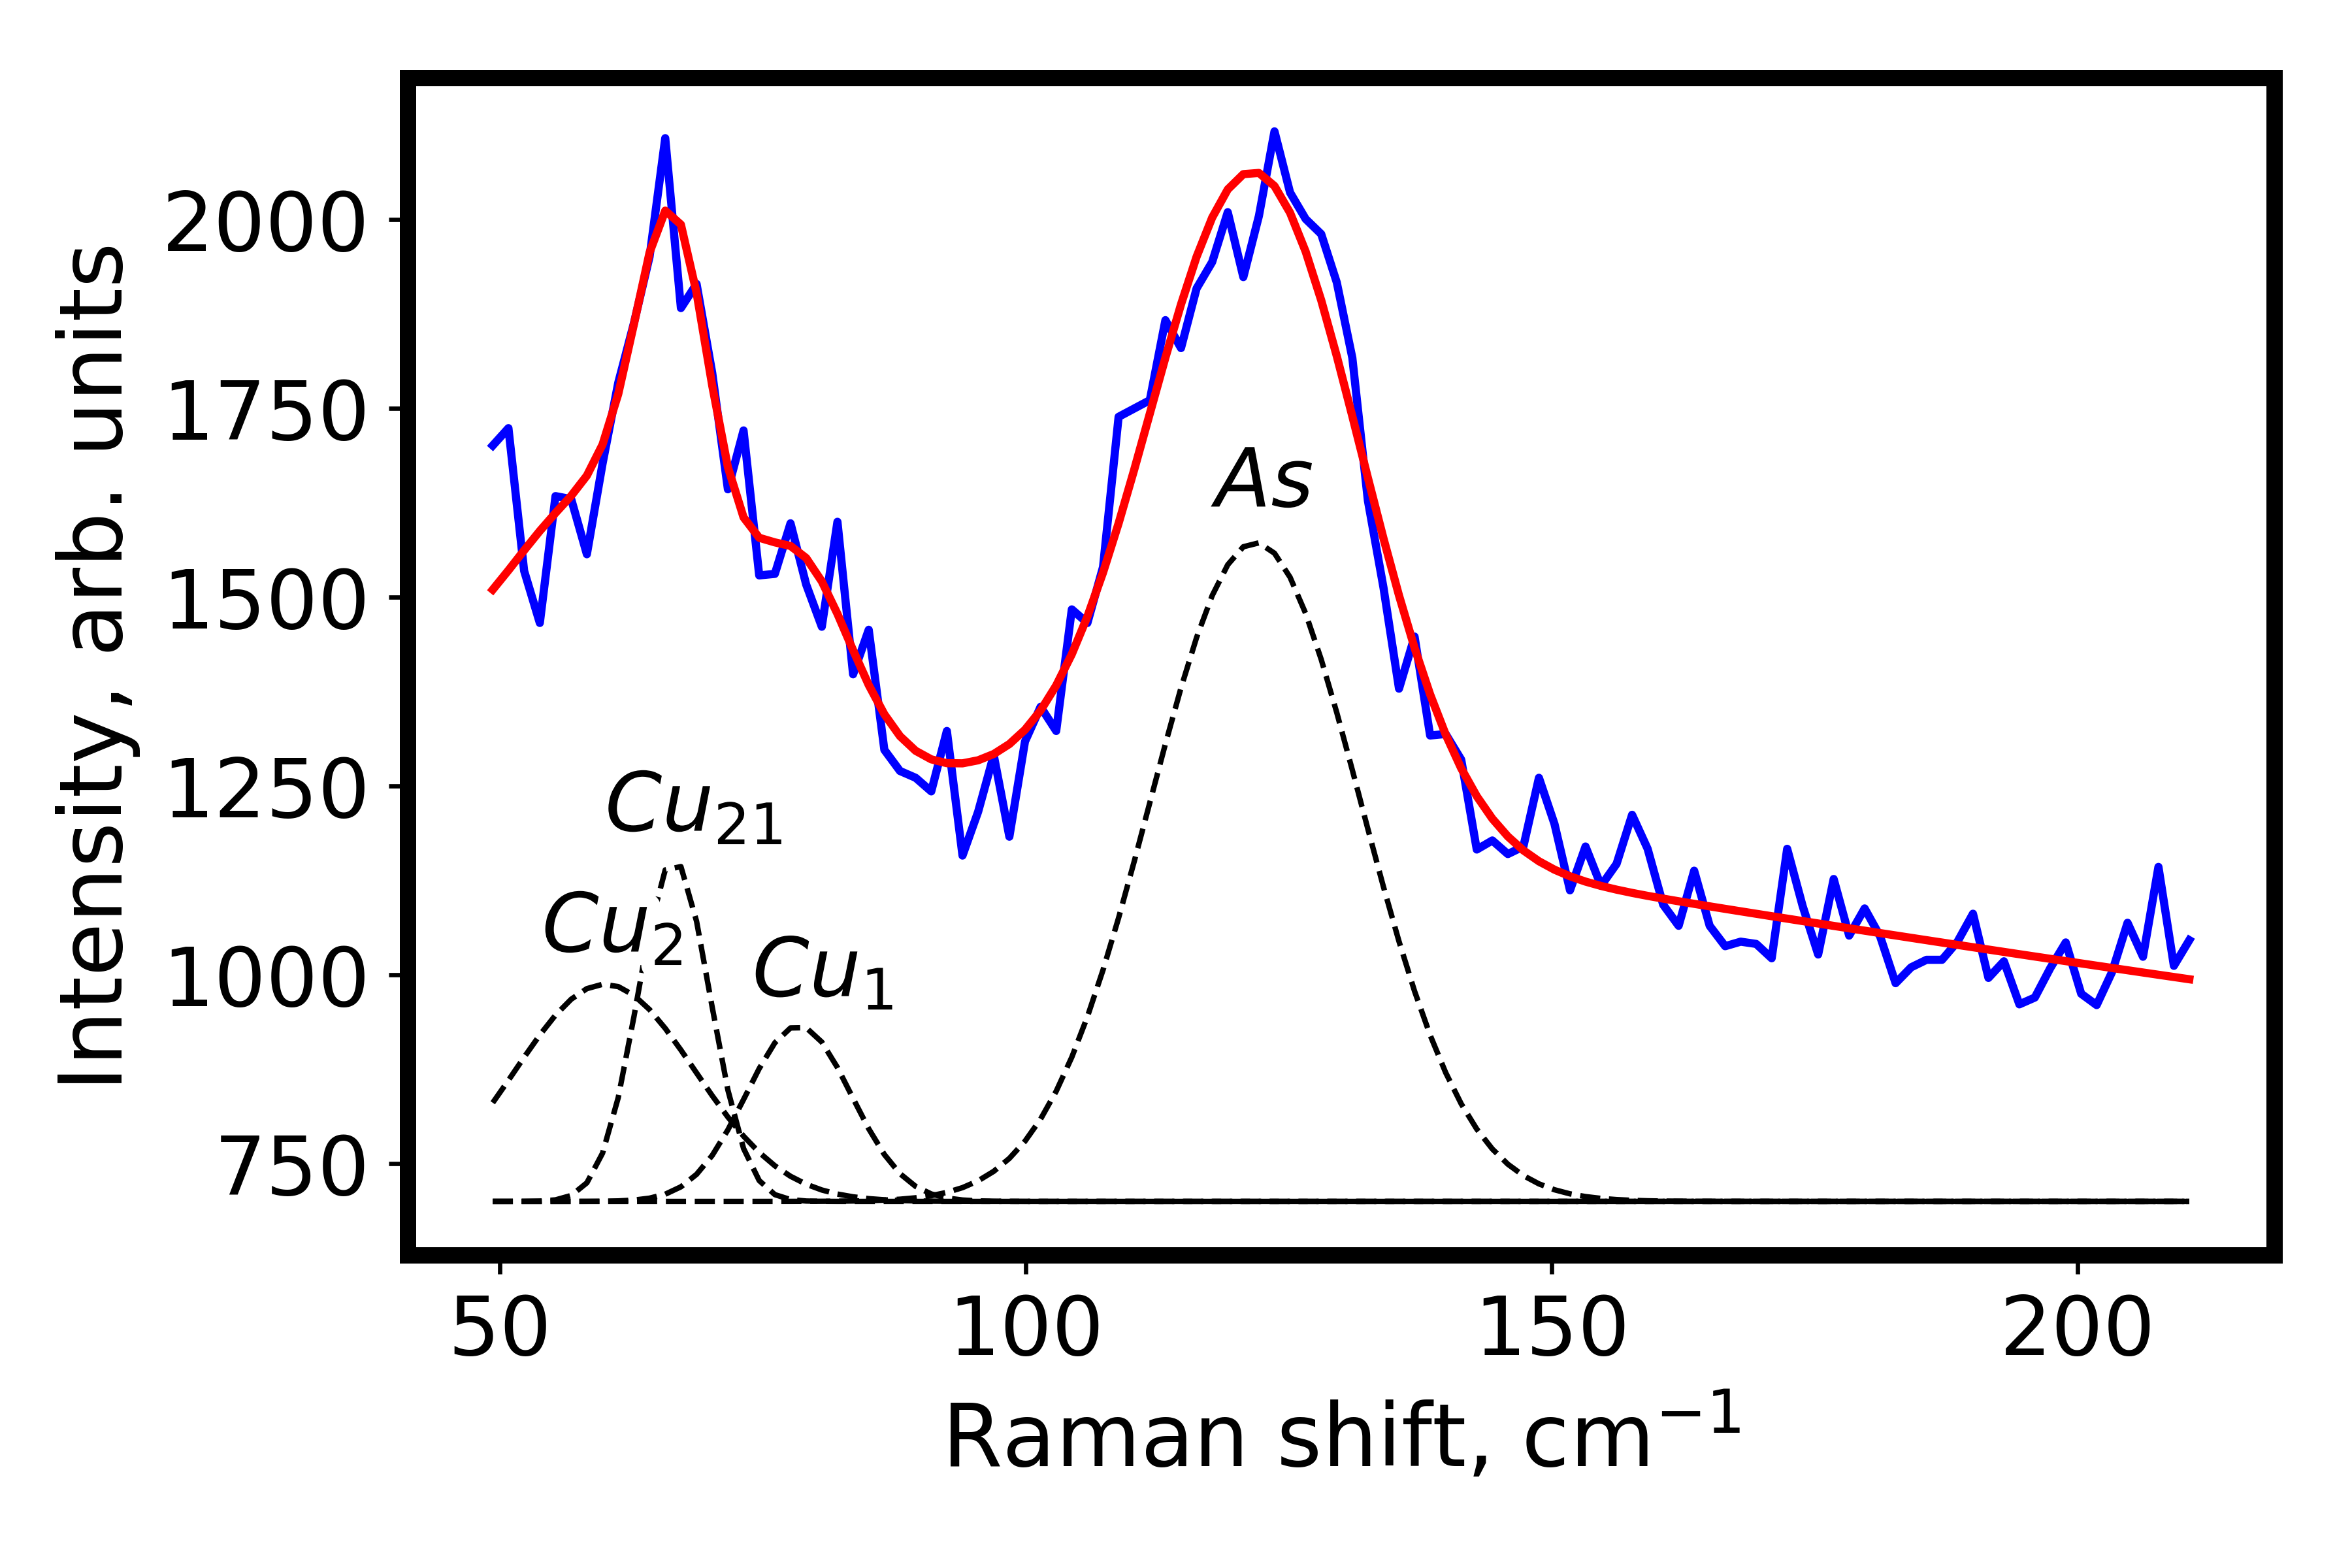
\includegraphics[width=0.48\textwidth]{raman_25_CuAsS3_low_energy}
\caption{\label{fig:low_energ_raman} Raman spectrum of the tennantite crystal  below 200 cm\textsuperscript{-1}. Experimental peaks are considered as the peaks with Einstein's energies. Blue --- experimental data, red --- modes based on the Einstein's energies fit, dotted --- fitted peaks.}
\end{figure}

\subsection{Theoretical analysis of possible polytypes and morphology of Laves polyhedra}\label{sec:level2}

Using the DFT calculations, we tested an assumption that the synthetic tennantite crystal structure is not the most energetically stable, and could  feature various polytypes.
As an initial point, we considered tennantite structure described in  \hmn{I -4 2 m}\ space group (henceforth called {\it reference structure}).
The unit cell contains Laves polyhedra formed by copper atoms around sulphur ones (Figure~\ref{fig:init_and_opt_laves}, number 0).
By shifting copper atoms by ca. 1~$\angstrom$, we produced a population of structures with varying shapes of Laves polyhedra, which were then subjected to the procedure of unconstrained structural optimization.
In the DFT calculations, where we cannot have Cu2 and Cu21 at the same time since we cannot have part of an atom occupying a position within a single polyhedron, we prefer to only use Cu2 notation, but distinguish their positions before and after optimization.
The Laves polyhedra morphologies before and after the optimization are shown in Figure~\ref{fig:init_and_opt_laves}.
Total energy differences between the reference structure of initial tennantite and optimized structures are shown in Figure~\ref{fig:energy_structure_rescale}.


\begin{figure}
\centering
 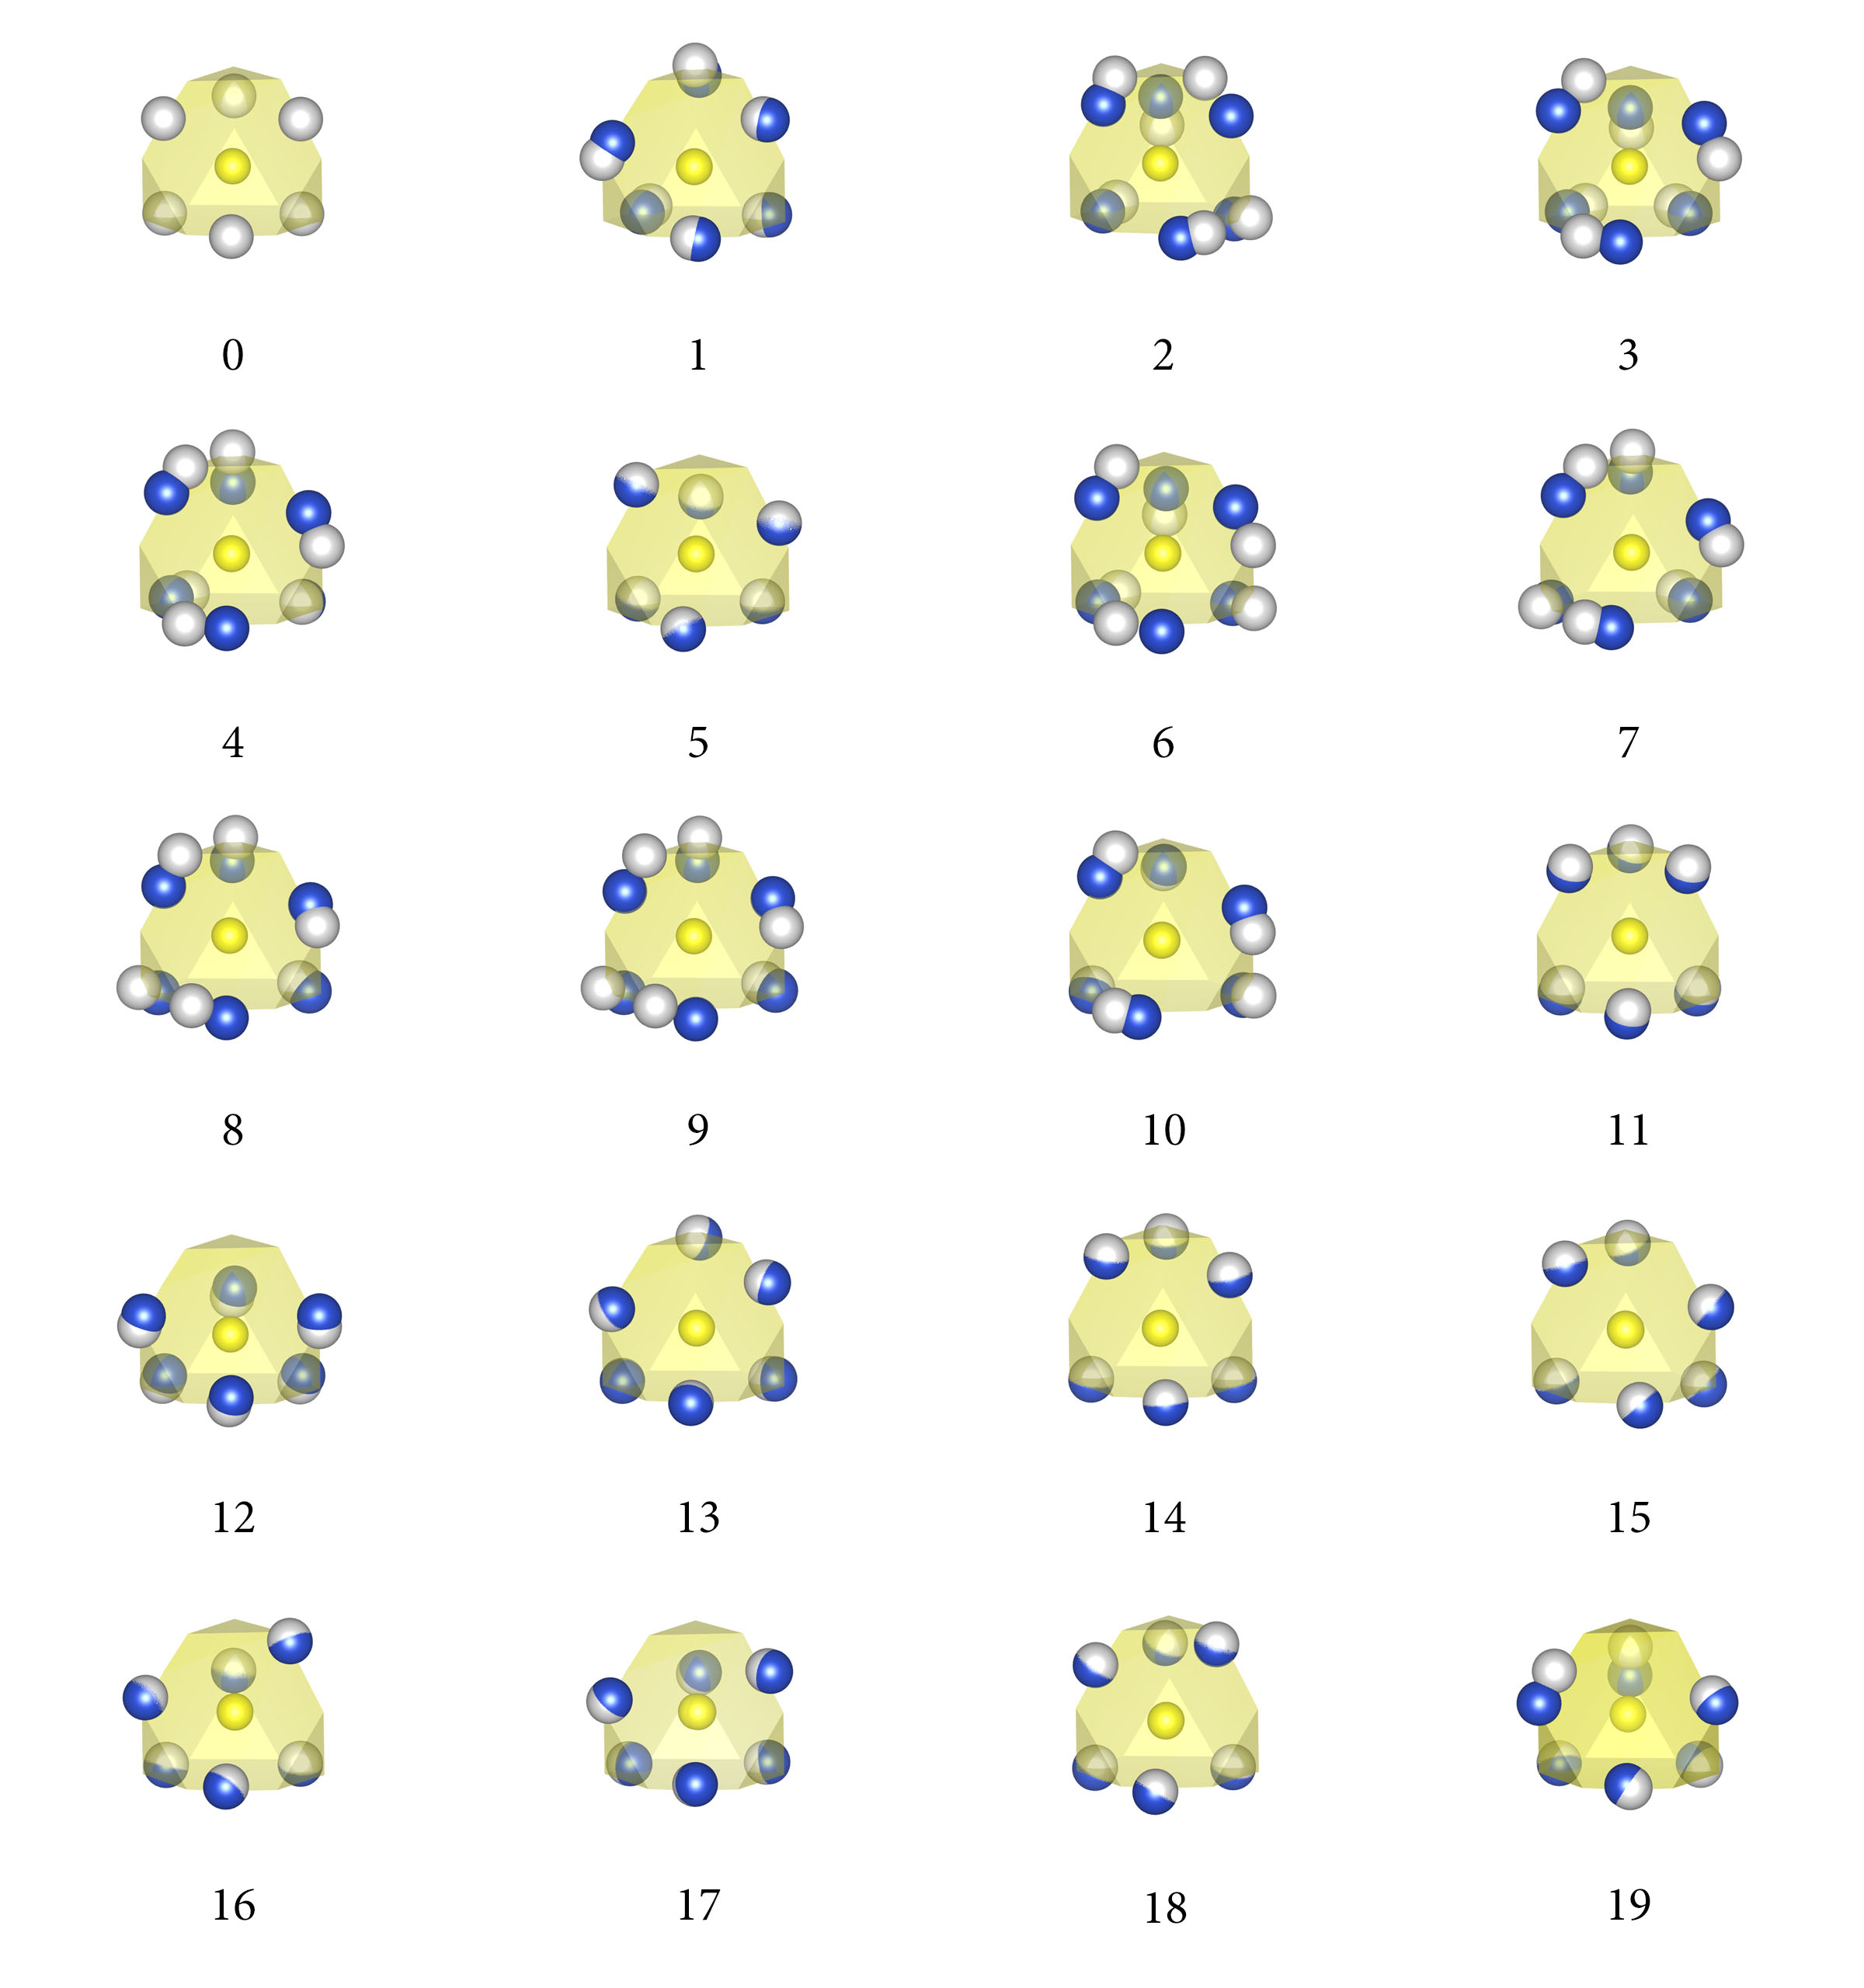
\includegraphics[width=0.48\textwidth]{Init_and_opt_renamed}
 \caption{\label{fig:init_and_opt_laves} The geometries of SCu\textsubscript{6} Laves polyhedra before and after structural optimization. sulphur atoms are shown in yellow, copper atoms before optimization are shown in grey, and after optimization in blue. VESTA\cite{Momma2011} was used for the visualisation. }
\end{figure}

Our calculations indicate that the experimentally determined synthetic tennantite structure is not the most energy favorable one at 0~K.

We observe 8 structures in our population with the energies less than the reference one.
They correspond to the structures No's 2, 3, 9, 11, 14, 17, 18, and 19, with the last one  possessing the lowest energy.
The coordination of the central sulphur atom deviates quite a lot from an ideal octahedron, with the energy gain being achieved by shifting one (structure 9), two (structures 17, 18), or three (structures 2, 3, 11, 14, 19) atoms.

%\begin{table}[h]%The best place to locate the table environment is directly after its first reference in text
%\caption{\label{tab:energy}%
%Anisotropic extinction parameters in Cu\textsubscript{12}As\textsubscript{4}S\textsubscript{13}.
%}
%\begin{ruledtabular}
%\begin{tabular}{cccc}
%Structure, number & Energy. eV & Structure, number & Energy, eV \\
%\colrule
%0   &   0.00 & 10   &  0.16 \\
%1   &   0.23 & 11   & -0.02 \\
%2   &  -0.02 & 12   &  0.05 \\
%3   &  -0.02 & 13   &  0.03 \\
%4   &   0.05 & 14   & -0.02 \\
%5   &   0.13 & 15   &  0.02 \\
%6   &  -0.00 & 16   &  0.12 \\
%7   &   0.23 & 17   & -0.02 \\
%8   &   0.06 & 18   & -0.03 \\
%9   &  -0.01 & 19   & -0.04 \\
%
%\end{tabular}
%\end{ruledtabular}
%\end{table}

\begin{table*}
\caption{\label{tab:energy}%
The difference between the reference structure energy, and the unit cell energy of tennantite with different Laves polyhedra.
}
\centering
\resizebox{\textwidth}{!}{
\begin{tabular}{ccccccccccc}
Structure, number & 0 & 1 & 2 & 3 & 4 & 5 & 6 & 7 & 8 & 9 \\
The difference of unit cells energies, eV &  0.00 &  0.23 & -0.02 & -0.02 &  0.05 &  0.13 & -0.00 &  0.23 &  0.06 & -0.01 \\
 \\
Structure, number & 10 & 11 & 12 & 13 & 14 & 15 & 16 & 17 & 18 & 19 \\
The difference of unit cells energies, eV &  0.16 & -0.02 &  0.05 &  0.03 & -0.02 &  0.02 &  0.12 & -0.02 & -0.03 & -0.04  \\
\end{tabular}}
\end{table*}

The analysis  of atomic charge distribution shows that the optimized structures can be divided into three groups: 1) with As charge of ca. $+3$ (reference compound also falls into this category), 2) with As charge less than $+1$, and 3) with intermediate As charge (between ca. $+1$ and $+2$).
Charge density on arsenic affects substantially the respective charge density at 1st sulphur position (see~Supplementary Material), and has a minor effect on Cu2 charges, while Cu1 is virtually unaffected by any change.
The other sulphur atom shows minor charge fluctuations, and they appear to be not directly associated with the oxidation state of arsenic.

\begin{figure}
\centering
 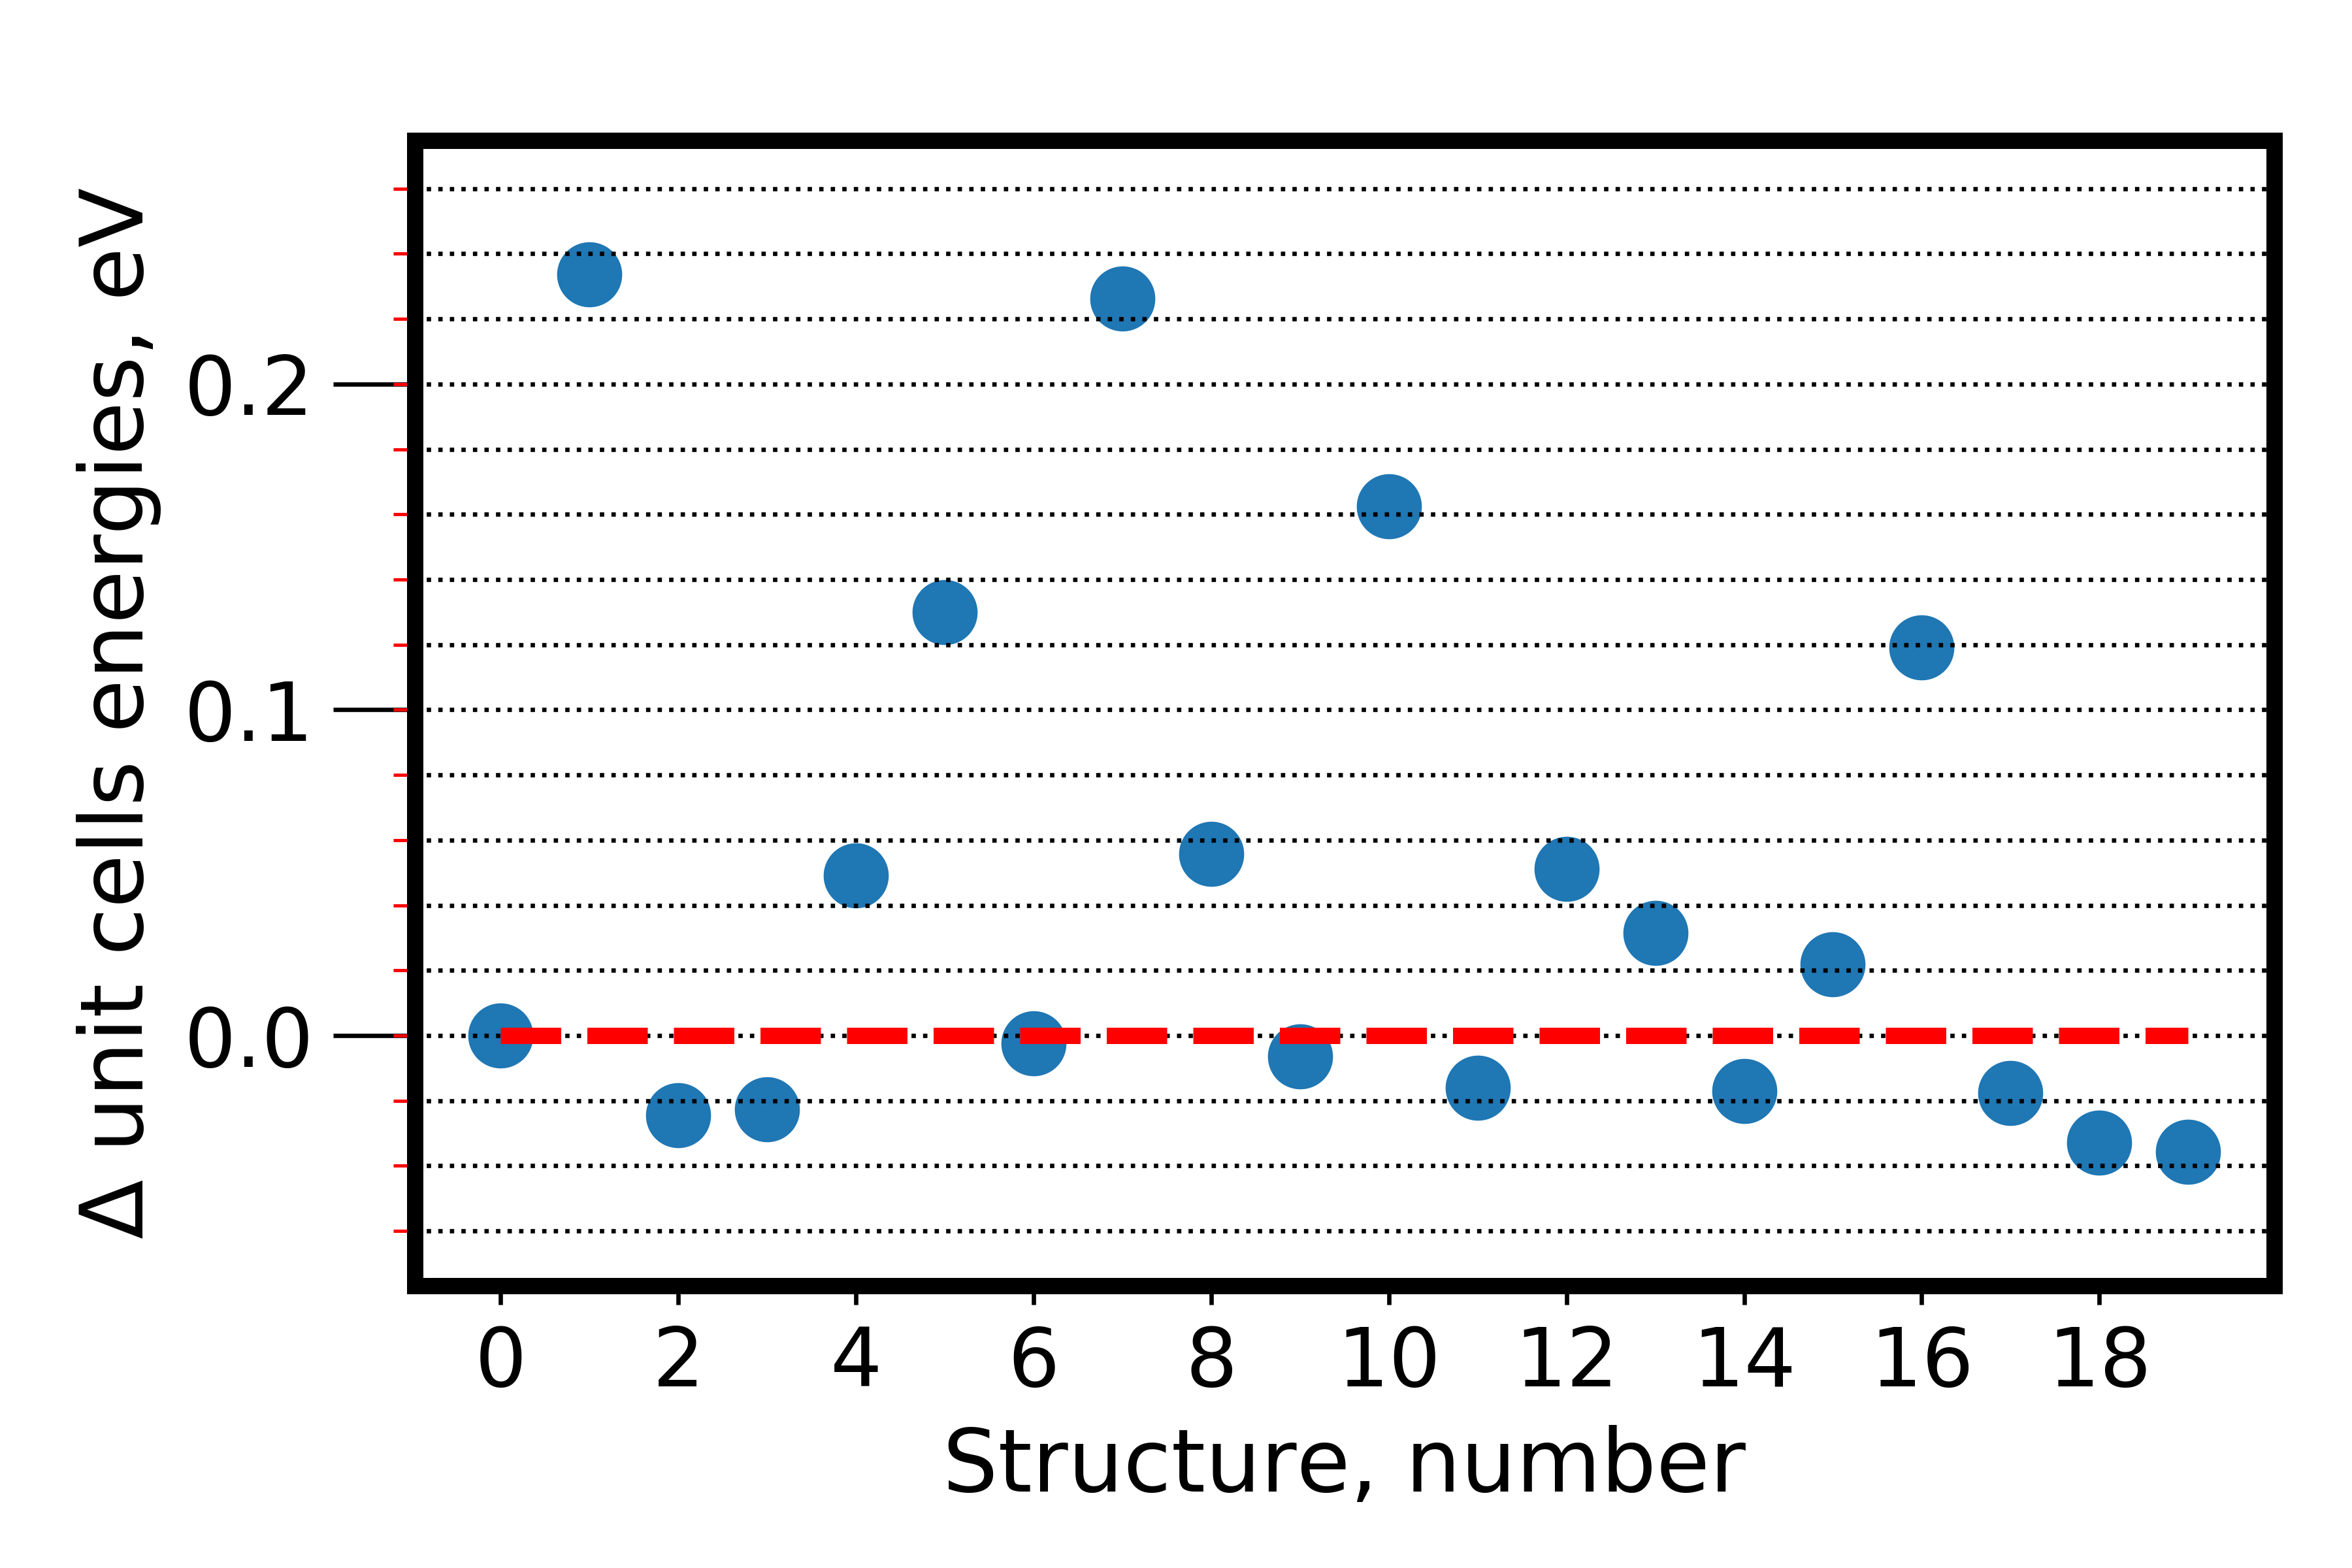
\includegraphics[width=0.48\textwidth]{energy_structure_rescale_ri}
 \caption{\label{fig:energy_structure_rescale} The difference between the reference structure energy and the unit cell energy of tennantite with different Laves polyhedra. Horizontal red line shows the reference unit cell energy. }
\end{figure}

Each of these groups has structures with an energy gain over the reference structure, and each of them has a certain split of a positive charge on Cu2 atoms, while Cu1 atomic charges remain constant throughout.
Thus, we can say that the splitting of the Cu2 position into Cu2 and Cu21, as evident from the XRD structure analysis, facilitates the differences in charge distribution.
Hence, the energy gain from forming Cu21 position leads to slightly different electronic states of Cu2 and Cu21 atoms, which, in turn, leads to the formation of asymmetric bonds, as was pointed out for tetrahedrites\cite{Lai2015,Long2020}.
We can also observe certain similarities between tennantite and inorganic compounds featuring atoms with  {\it 3d\textsuperscript{9}}  configuration, and having asymmetric Fermi surface.
The resulting complex charge distribution, and variances in the copper atom charges and, therefore, effective oxidation states, caused by structural shifts, may, in turn, be the reason for complex exchange interactions and the reported AFM ordering\cite{yaroslavzev2019} in tennantite.
Moreover, the same structure features have been described for tetrahedrite\cite{DiPaola2020}.
The authors noted, that understanding these features provides a key to descriptions of the phonon-limited electrical resistivity, and the Lorenz number.

It must be noted that the majority of the favorable structures belongs to group 2, i.e. more covalent structures with both arsenic and sulphur atoms showing relatively low positive and negative charges, respectively.
Interestingly, the reference structure is significantly more ionic in this respect.
Also, we must point out that, according to the DFT calculations, several structures have energy minimum within hundredths of eV (Table~\ref{tab:energy}), i.e. only several~kJ/mol (1~eV~$\sim$~96.5 kJ/mol), which is on the limit of the accuracy of the method.
This indicates, that the tennantite experimental structure may be an averaged result of several variations of the copper atoms shifts.


\section{Conclusions}\label{sec:level1}
In conclusion, using a combination of several experimental techniques, we have investigated the structural variations of synthetic tennantite, Cu\textsubscript{12}As\textsubscript{4}S\textsubscript{13}, manifesting itself as a dynamic disorder of the copper atoms.
The tennantite structure tends to conform to the asymmetric covalent polar bonds and its charge distribution is significantly affected by the atomic shifts in Laves polyhedra.
These effects, in turn, give rise to the out-of-plane low frequency rattling modes, well described by Einstein characteristic temperatures: 74, 104, 115, and 185~K.
The peculiarities of the tennantite crystal and electronic structure, including lattice dynamics and shifting charge distribution, shows similarities between this compound and inorganic compounds with an asymmetric Fermi surface, thus making tennantite--tetrahedrite group attractive research objects.

Our extensive structural studies revealed a strong tendency of anisotropic shifts in electron density of the bulk sample, with no evidence of a distortion or local defects.

The specially-designed technique was successfully tested for the experimental ADP analysis, and, as we have demonstrated, can be used as a new method of the experimental study of a crystal structure.

\section{Acknowledgments}\label{sec:level1}
This research was partially supported by Russian Science Foundation (Grant No. 19-13-00451). The calculations were carried out using the equipment of the shared research facilities of the HPC computing resources at Lomonosov Moscow State University.
X-ray diffraction study was performed using the equipment of the Shared Research Center FSRC “Crystallography and Photonics” RAS and was supported by the Ministry of  Science and Higher Education of the Russian Federation (project RFMEFI62119X0035). X-ray diffraction part of this work was supported by the Ministry of Science and Higher Education of the Russian Federation within the State assignment  of the Federal Scientific Research Center “Crystallography and Photonics” of the Russian Academy of Sciences.
Electron microscopy was carried out using the equipment of the Resource Centre “Nanozond“
National Research Center “Kurchatov Institute“.
We thank I. A. Perezhogin for valuable comments and  Professor A. N. Babushkin for the tennantite ingot.


\section{References}\label{sec:level1}
\bibliographystyle{elsarticle-num}
\bibliography{reff}

\end{document}
\endinput
%%
%% End of file `elsarticle-template-num.tex'.
